\documentclass[12pt]{article}\usepackage[]{graphicx}\usepackage[]{color}
% maxwidth is the original width if it is less than linewidth
% otherwise use linewidth (to make sure the graphics do not exceed the margin)
\makeatletter
\def\maxwidth{ %
  \ifdim\Gin@nat@width>\linewidth
    \linewidth
  \else
    \Gin@nat@width
  \fi
}
\makeatother

\definecolor{fgcolor}{rgb}{0.345, 0.345, 0.345}
\newcommand{\hlnum}[1]{\textcolor[rgb]{0.686,0.059,0.569}{#1}}%
\newcommand{\hlstr}[1]{\textcolor[rgb]{0.192,0.494,0.8}{#1}}%
\newcommand{\hlcom}[1]{\textcolor[rgb]{0.678,0.584,0.686}{\textit{#1}}}%
\newcommand{\hlopt}[1]{\textcolor[rgb]{0,0,0}{#1}}%
\newcommand{\hlstd}[1]{\textcolor[rgb]{0.345,0.345,0.345}{#1}}%
\newcommand{\hlkwa}[1]{\textcolor[rgb]{0.161,0.373,0.58}{\textbf{#1}}}%
\newcommand{\hlkwb}[1]{\textcolor[rgb]{0.69,0.353,0.396}{#1}}%
\newcommand{\hlkwc}[1]{\textcolor[rgb]{0.333,0.667,0.333}{#1}}%
\newcommand{\hlkwd}[1]{\textcolor[rgb]{0.737,0.353,0.396}{\textbf{#1}}}%
\let\hlipl\hlkwb

\usepackage{framed}
\makeatletter
\newenvironment{kframe}{%
 \def\at@end@of@kframe{}%
 \ifinner\ifhmode%
  \def\at@end@of@kframe{\end{minipage}}%
  \begin{minipage}{\columnwidth}%
 \fi\fi%
 \def\FrameCommand##1{\hskip\@totalleftmargin \hskip-\fboxsep
 \colorbox{shadecolor}{##1}\hskip-\fboxsep
     % There is no \\@totalrightmargin, so:
     \hskip-\linewidth \hskip-\@totalleftmargin \hskip\columnwidth}%
 \MakeFramed {\advance\hsize-\width
   \@totalleftmargin\z@ \linewidth\hsize
   \@setminipage}}%
 {\par\unskip\endMakeFramed%
 \at@end@of@kframe}
\makeatother

\definecolor{shadecolor}{rgb}{.97, .97, .97}
\definecolor{messagecolor}{rgb}{0, 0, 0}
\definecolor{warningcolor}{rgb}{1, 0, 1}
\definecolor{errorcolor}{rgb}{1, 0, 0}
\newenvironment{knitrout}{}{} % an empty environment to be redefined in TeX

\usepackage{alltt}
\usepackage[utf8]{inputenc}
\usepackage[german]{babel}
\usepackage{apacite}
\usepackage{graphicx}
\usepackage{amsmath}
\usepackage{xcolor}
\usepackage{a4wide}
\usepackage[nottoc, numbib]{tocbibind}
\usepackage{natbib} 
\usepackage{booktabs}
\usepackage{longtable}
\usepackage{array}
\usepackage{multirow}
\usepackage{wrapfig}
\usepackage{float}
\usepackage{colortbl}
\usepackage{pdflscape}
\usepackage{tabu}
\usepackage{threeparttable}
\usepackage{threeparttablex}
\usepackage[normalem]{ulem}
\usepackage{makecell}
\usepackage{siunitx}
\usepackage[singlelinecheck=false, labelfont=bf]{caption}
\usepackage{setspace}
\usepackage{rotating}
\captionsetup{font=footnotesize}



\makeatletter
\let\save@mathaccent\mathaccent
\newcommand*\if@single[3]{%
  \setbox0\hbox{${\mathaccent"0362{#1}}^H$}%
  \setbox2\hbox{${\mathaccent"0362{\kern0pt#1}}^H$}%
  \ifdim\ht0=\ht2 #3\else #2\fi
  }
%The bar will be moved to the right by a half of \macc@kerna, which is computed by amsmath:
\newcommand*\rel@kern[1]{\kern#1\dimexpr\macc@kerna}
%If there's a superscript following the bar, then no negative kern may follow the bar;
%an additional {} makes sure that the superscript is high enough in this case:
\newcommand*\widebar[1]{\@ifnextchar^{{\wide@bar{#1}{0}}}{\wide@bar{#1}{1}}}
%Use a separate algorithm for single symbols:
\newcommand*\wide@bar[2]{\if@single{#1}{\wide@bar@{#1}{#2}{1}}{\wide@bar@{#1}{#2}{2}}}
\newcommand*\wide@bar@[3]{%
  \begingroup
  \def\mathaccent##1##2{%
%Enable nesting of accents:
    \let\mathaccent\save@mathaccent
%If there's more than a single symbol, use the first character instead (see below):
    \if#32 \let\macc@nucleus\first@char \fi
%Determine the italic correction:
    \setbox\z@\hbox{$\macc@style{\macc@nucleus}_{}$}%
    \setbox\tw@\hbox{$\macc@style{\macc@nucleus}{}_{}$}%
    \dimen@\wd\tw@
    \advance\dimen@-\wd\z@
%Now \dimen@ is the italic correction of the symbol.
    \divide\dimen@ 3
    \@tempdima\wd\tw@
    \advance\@tempdima-\scriptspace
%Now \@tempdima is the width of the symbol.
    \divide\@tempdima 10
    \advance\dimen@-\@tempdima
%Now \dimen@ = (italic correction / 3) - (Breite / 10)
    \ifdim\dimen@>\z@ \dimen@0pt\fi
%The bar will be shortened in the case \dimen@<0 !
    \rel@kern{0.6}\kern-\dimen@
    \if#31
      \overline{\rel@kern{-0.6}\kern\dimen@\macc@nucleus\rel@kern{0.4}\kern\dimen@}%
      \advance\dimen@0.4\dimexpr\macc@kerna
%Place the combined final kern (-\dimen@) if it is >0 or if a superscript follows:
      \let\final@kern#2%
      \ifdim\dimen@<\z@ \let\final@kern1\fi
      \if\final@kern1 \kern-\dimen@\fi
    \else
      \overline{\rel@kern{-0.6}\kern\dimen@#1}%
    \fi
  }%
  \macc@depth\@ne
  \let\math@bgroup\@empty \let\math@egroup\macc@set@skewchar
  \mathsurround\z@ \frozen@everymath{\mathgroup\macc@group\relax}%
  \macc@set@skewchar\relax
  \let\mathaccentV\macc@nested@a
%The following initialises \macc@kerna and calls \mathaccent:
  \if#31
    \macc@nested@a\relax111{#1}%
  \else
%If the argument consists of more than one symbol, and if the first token is
%a letter, use that letter for the computations:
    \def\gobble@till@marker##1\endmarker{}%
    \futurelet\first@char\gobble@till@marker#1\endmarker
    \ifcat\noexpand\first@char A\else
      \def\first@char{}%
    \fi
    \macc@nested@a\relax111{\first@char}%
  \fi
  \endgroup
}
\makeatother
\newcommand\test[1]{%
$#1{M}$ $#1{A}$ $#1{g}$ $#1{\beta}$ $#1{\mathcal A}^q$
$#1{AB}^\sigma$ $#1{H}^C$ $#1{\sin z}$ $#1{W}_n$}



\title{Schätzgenauigkeit von Standardfehlern und deren Einfluss auf die Zuverlässigkeit von Tests bei der Analyse von hierarchischen Daten \\ \large{Ein Vergleich zwischen linearen und hierarchischen linearen Modellen}}

\author{Masterarbeit von \\ Noah Bosshart \\ Mat-Nr.: 13-747-141 \\ \\ \\ Betreut durch \\ Prof. Dr. Carolin Strobl}
\IfFileExists{upquote.sty}{\usepackage{upquote}}{}
\begin{document}
\setstretch{1.5}

\begin{figure}[t]
  \centering
  
\includegraphics[width = 8cm]{uzh_logo}
\end{figure}

\maketitle
\thispagestyle{empty}

\newpage
\pagenumbering{Roman}
\tableofcontents

\newpage
\listoffigures

\newpage
\listoftables
\newpage


\section*{Kurzfassung}
Diese Arbeit kombiniert eine theoretische Einführung in die hierarchischen linearen Modelle (HLM) und  eine Simulationsstudie über deren Schätzgenauigkeit. In der theoretischen Einführung wird erklärt, was hierarchische Daten sind und was für Konsequenzen eine ungenügende Berücksichtigung dieser Datenstrukturen mit sich bringen. Dabei wird konkret auf den problematischen Einsatz von normalen linearen Modellen (LM) zur Analyse von solchen Daten eingegangen und wie ein HLM diese Probleme umgehen kann. In einer Simulationsstudie wurde untersucht, wie sich die Ausprägung der Intraklassen Korrelation (IKK) und das Level der Intervention auf die Schätzgenauigkeit von LMs und HLMs auswirkt. Dabei zeigte sich, dass beide Modelle in allen Bedingungen die Regressionskoeffizienten genau schätzten. Der Standardfehler wurde allerdings von LMs mit zunehmender IKK ungenauer geschätzt, wobei die Schätzung von HLMs genau blieb. Diese ungenaue Schätzung des Standardfehlers durch ein LM führte in Abhängigkeit des Studiendesign zu einer Reduktion der Power oder einer Erhöhung der Fehler Typ 1 Rate. So wurde bei einer Intervention auf Level-1 der Standardfehler durch ein LM bei steigender IKK zunehmend überschätzt. Dies resultierte in einer abnehmenden Power des LMs. Der Standardfehler einer Level-2 Variable wurden von LMs hingegen zunehmend unterschätzt, was schlussendlich in einer erhöhten Fehler Typ 1 Rate resultierte. Dabei litt ein HLM unter keiner dieser Limitationen und wies eine adäqute Fehler Typ 1 Rate sowie eine zuverlässige Power auf. Diese Studie konnte zum einen Ergebnisse aus früheren Studien replizieren und zum anderen aufzeigen, dass ein HLM bei der Analyse von hierarchischen Daten zu genaueren Ergebnissen führt.




\newpage

\pagenumbering{arabic}
\section{Einleitung}
Hierarchische Daten treten häufig in den Sozialwissenschaften auf, unter anderem auch in der Psychologie \citep{SnijdersTomA.B2012Ma:a}. Von hierarchischen Daten wird gesprochen, wenn beispielsweise Daten von Schulkindern innerhalb verschiedener Schulklassen oder von Mitarbeitenden aus mehreren Teams erhoben werden. Aber auch Daten aus Langzeitstudien werden als gruppiert bezeichnet, da mehrere Messzeitpunkte innerhalb einer Person gruppiert sind. Hierarchische Daten werden in Levels unterteilt, wobei Daten aus der niedrigsten Stufe als Level-1 Einheiten bezeichnet werden \citep{SnijdersTomA.B2012Ma:a}. Ein Beispiel für Level-1 Einheiten sind Schulkinder. Diese Schulkinder befinden sich wiederum in Klassen, die in der Hierarchiestufe höher sind und folglich als Level-2 Einheiten bezeichnet werden. Würde man nun in einer Studie nicht nur Schulkinder in Schulklassen, sondern auch  die Schulen selbst berücksichtigen, würden die Schulen als Level-3 Einheit bezeichnet werden. Die Anzahl der Levels könnte man theoretisch beliebig hoch wählen, solange es das Studiendesign erlaubt und es aus der Perspektive der Forschungsfrage sinnvoll ist. Der Einfachheit halber beschränken wir uns im Laufe dieser Arbeit aber auf hierarchische Daten mit zwei Levels. In Tabelle \ref{tab:beispiele_levels} werden einige Beispiele für Level-1 und Level-2 Einheiten aufgeführt. 
\begin{table}[b!]
\centering
\begin{threeparttable}
\caption{Beispiele für Level-1 und Level-2 Einheiten}
\begin{tabular}{ll}
\toprule
Level-1 				& Level-2 	\\
\midrule
Schulkinder 			& Klasse 	\\
Studierende 			& Studienrichtungen \\
Kinder 					& Familien 	\\
Familien 				& Nachbarschaften \\
Mitarbeitende			& Teams \\
Teams					& Unternehmen \\
Behandelte Personen	 	& Therapierende \\
Therapierende 			& Kliniken \\
Mehrere Messzeitpunkte 	& Person \\
\bottomrule
\end{tabular}
\label{tab:beispiele_levels}
\end{threeparttable}
\end{table}
Dabei ist zu beachten, dass sich das Level derselben Einheit je nach Untersuchungsgegenstand ändern kann. Wie man in der Tabelle \ref{tab:beispiele_levels} erkennen kann, sind Familien einmal als Level-1 und einmal als Level-2 Einheit aufgeführt. Daher ist es wichtig die Level Bezeichnung nicht als starr zu betrachtet. Vielmehr sollte man sich grundsätzlich an den niedrigsten Einheiten im Datensatz orientieren. Diesen Einheiten wird dann das Level-1 zugeschrieben.

In der Forschung ist es aus Kostengründen oder aus Gründen des Studiendesigns oft nicht möglich, solche gruppierte Datenstrukturen zu vermeiden \citep{SnijdersTomA.B2012Ma:a, woltman2012introduction}. Als eine von vielen Ursachen, die zur Entstehung solcher Datenstrukturen führt, nennen Snijders und Bosker \citeyearpar{SnijdersTomA.B2012Ma:a} \textit{Multistage Sampling}. Unter \textit{Multistage Sampling} versteht man, dass die Forschenden in der Datenerhebung auf in der Population vorhandene Gruppen zugreifen. So wäre es beispielsweise kostengünstiger eine Intervention mit 10 Schulkindern aus jeweils 100 Schulklassen durchzuführen, als mit einem Schulkind aus jeweils 1000 Schulklassen. Dadurch erhalten die Forschenden eine vermeintlich gleichgrosse Stichprobe von 1000 Beobachtungen, müssen die Intervention aber nur an 100 Schulklassen und nicht an 1000 durchführen. Dieses Auswahlverfahren führt aber dazu, dass die erhobenen Daten nicht mehr voneinander unabhängig sind. Werden nun aus jeder Schulklasse 10 Schulkinder für eine Studie ausgewählt, ist es sehr wahrscheinlich, dass Schulkinder aus derselben Klasse zueinander ähnlichere Leistungen erzielen werden. Dieser Zusammenhang kann auf unterschiedliche Ursache zurückzuführen sein. Beispielsweise könnte die didaktischen Fähigkeiten der Lehrpersonen oder die Lichtverhältnisse im Klassenzimmer einen Einfluss auf die Leistungen der Kinder aus derselben Klasse haben. 

Nach Snijders und Bosker \citeyearpar{SnijdersTomA.B2012Ma:a} gibt es unterschiedliche Formen, wie diese Einheiten zueinander in Beziehung stehen können. Ein Beispiel für einen Zusammenhang auf Level-1 wäre, dass die Lernmotivation eines Schulkindes sich auf seine schulische Leistung auswirkt. Aber auch Level-2 Einheiten können sich gegenseitig beeinflussen. Das Klima der Schulklasse könnte sich beispielsweise auf das Stressempfinden der Lehrperson auswirken. Hier wird von einem Zusammenhang innerhalb des Levels gesprochen, weil die unabhängige Variable (z.B. Lernmotivation, Klima der Schulklasse) auf dem gleichen Level wie die abhängige Variable (z.B. schulische Leistung, Stressempfinden) ist. Häufig ist es allerdings der Fall, dass es levelübergreifende Zusammenhänge zwischen den Einheiten gibt. So können beispielsweise die didaktischen Fähigkeiten einer Lehrperson (Level-2) und die Lernmotivation der Schulkinder (Level-1) die individuelle Leistung (Level-1) beeinflussen. Dieser Zusammenhang muss nicht zwingend direkt sein. Es kann auch vorkommen, dass die didaktischen Fähigkeiten den Zusammenhang zwischen Lernmotivation und individueller Leistung moderiert. In diesem Fall wird gemäss Snijders und Bosker \citeyearpar{SnijdersTomA.B2012Ma:a} von einer \textit{Cross-Level} Interaktion gesprochen.

Werden diese Abhängigkeiten in der Analyse nicht berücksichtigt, kann dies unter anderem zu einer erhöhten Fehler Typ 1 Rate führen \citep{dorman2008effect, mcneish2014analyzing}. Das heisst, dass Forschende vermehrt zu Fehlschlüssen bezüglich des Einflusses ihrer unabhängigen Variablen gelangen und irrtümlich annehmen, einen Effekt eines Verfahren gefunden zu haben, obwohl es diesen Effekt gar nicht gibt. Missachten dieser Abhängigkeiten kann aber nicht nur zu einer erhöhten Fehler Typ 1 Rate führen, sondern auch die Fehler Typ 2 Rate erhöhen \citep{MOERBEEK2003341}. Eine erhöhte Fehler Typ 2 Rate resultiert in einer niedrigeren Power einen Effekt zu entdecken, wenn dieser auch effektiv vorhanden ist. Das Vorhandensein von hierarchischen Daten ist allerdings kein unlösbares Problem. Mit Analyseansätzen, die diese hierarchische Struktur der Daten berücksichtigen, lassen sich solche erhöhten Fehler Typ 1 und 2 Raten vermeiden. Einer dieser Ansätze der Multilevel Analyse ist das hierarchische lineare Modell, das im Fokus dieser Arbeit steht.

Diese Arbeit ist in zwei Teile unterteilt. Im ersten Teil wird das Konzept und die Theorie der Multilevel Analyse behandelt. Dabei wird kurz auf die verschiedenen Methoden eingegangen, wie man Daten auf ihre hierarchische Struktur überprüfen kann. Anschliessend wird das hierarchische lineare Modell vorgestellt und wie genau solche Modelle aufgebaut sind. Darauf folgend wird die Anwendung dieser Methoden in der Statistikumgebung R besprochen \citep{R}. Im zweiten Abschnitt dieser Arbeit wird eine Simulationsstudie durchgeführt, deren Ziel es ist, bereits vorhandene Ergebnisse in der Literatur zu replizieren und zu illustrieren, dass eine Multilevel Analyse bei hierarchischen Daten verlässliche Resultate liefert. Begleitend zu dieser Studie wird eine Shiny App programmiert \citep{shiny}, die zum einen das Konzept der Multilevel Analyse visualisiert und die Ergebnisse der hier durchgeführten Simulationsstudie interaktiv abbildet.

\section{Konzept und Anwendung von Multilevel Analyse}
Wie in der Einleitung erläutert wurde, gibt es viele Situationen in denen hierarchische Daten vorhanden sind und man zu Fehlschlüssen gelangen kann, wenn man diese Strukturen nicht berücksichtigt. In diesem Abschnitt wird nun etwas genauer auf das Konzept und die dahintersteckende Theorie der Multilevel Analyse eingegangen. Dazu wird zuerst ein simulierter Beispieldatensatz vorgestellt, anhand dessen die besprochenen Modelle erklärt werden. Als erstes wird auf die Probleme eingegangen, die durch die Verwendung von einfachen linearen Modellen (LM) entstehen. Anschliessend wird das hierarchische lineare Modell (HLM) als das zugrundeliegende statistische Modell der Multilevel Analyse eingeführt. Das HLM gilt als eine Erweiterung der einfachen LM \citep{SnijdersTomA.B2012Ma:a}. Dabei werden bei HLM in \textit{Random Intercept} und \textit{Random Intercept and Slope} Modelle unterschieden. Es werden beide Modellformen besprochen und dabei wird erläutert wie die beiden Faktoren Achsenabschnitt (engl. \textit{Intercept}) und Steigung (engl. \textit{Slope}) zusammenhängen. Nachdem die verschiedenen Formen von HLM besprochen worden sind, wird in einem etwas praktischeren Teil die Anwendung von Multilevel Analyse in R anhand von Beispielen etwas näher gebracht.

\subsection{Beispiel zur Theorie} \label{section:bsp_theorie}
In den folgenden Abschnitten wird die Theorie zur Analyse von hierarchischen Daten anhand eines Beispieldatensatzes erläutert. Bei dem Beispiel handelt es sich um insgesamt 150 Schulkindern aus 5 Schulklassen, die eine Mathematikprüfung geschrieben haben. Neben der erreichten Punktzahl wurde für jedes Kind zufällig ein Geschlecht, die Anzahl an gelöster Übungen, einen Wert für sozioökonomische Status und einen Intelligenzquotienten simuliert. Auf Stufe der Klasse wurden ausserdem noch die Anzahl Fenster im Klassenzimmer simuliert. Da dieser Datensatz selbst generiert wurde und aus keiner Studie entstammt, sollten Ergebnisse, die aus diesen Berechnungen entstehen nicht weiter interpretiert werden. In Tabelle \ref{tab:beispiel_theorie} sind zur Veranschaulichung dieser Daten eine Auswahl von 10 Schulkindern aufgeführt.
\begin{table}[t!]
\centering
\begin{threeparttable}
\caption{Ausschnitt des simulierten Datensatzes} 
\begin{tabular}{cccccccc}
  \toprule
 Schulkind Nr. & Klasse & Übungen & Punktzahl & Geschlecht & Anz. Fenster & SES & IQ \\ 
  \midrule
101 & 4 & 17 & 21 & m & 3 & 16 & 104 \\ 
  75 & 3 & 7 & 29 & m & 8 & 27 & 112 \\ 
  126 & 5 & 23 & 26 & w & 4 & 14 & 110 \\ 
  14 & 1 & 10 & 29 & m & 4 & 21 & 84 \\ 
  137 & 5 & 16 & 18 & w & 4 & 17 & 109 \\ 
  100 & 4 & 7 & 16 & w & 3 & 20 & 98 \\ 
  78 & 3 & 28 & 44 & w & 8 & 23 & 105 \\ 
  121 & 5 & 25 & 33 & w & 4 & 21 & 99 \\ 
  16 & 1 & 7 & 24 & w & 4 & 30 & 77 \\ 
  116 & 4 & 14 & 29 & m & 3 & 19 & 90 \\ 
   \bottomrule
\end{tabular}
\label{tab:beispiel_theorie}
\end{threeparttable}
\end{table}

Betrachtet man die Variablen des Datensatzes, kann man erkennen, dass es sich um einen hierarchischen Datensatz mit zwei Levels handelt. Zu den Level-1 Variablen gehören alle Variablen die sich auf der Stufe der tiefsten Einheit (Schulkinder) befinden. Dazu zählen die Anzahl gelösten Übungen, die erreichte Punktzahl, das Geschlecht, der sozioökonomische Status und der IQ. Die beiden anderen Variablen Klasse und die Anzahl Fenster im Klassenzimmer gehören zur Level-2 Ebene. Durch ein kurzes Betrachten der Daten, kann man also relativ schnell herausfinden, ob es sich um einen hierarchischen Datensatz handelt. Allerdings gibt uns diese Betrachtung der Daten keine Auskunft darüber, ob und wie stark die Gruppenzugehörigkeit (Klasse) einen Einfluss auf die erreichte Punktzahl in der Mathematikprüfung hat. Die Intraklassen Korrelation kann diesbezüglich mehr Klarheit schaffen und wird im nächsten Abschnitt vorgestellt.


\subsection{Intraklassen Korrelation} \label{section:icc}
Der Einfluss einer hierarchischen Struktur auf eine abhängige Variable kann durch die Intraklassen Korrelation (IKK) beschrieben werden. Die IKK beschreibt den Grad der Ähnlichkeit von Level-1 Einheiten innerhalb einer Level-2 Einheit und kann als Verhältnis der Varianz zwischen den Level-2 Einheiten und der Gesamtvarianz beschrieben werden \citep{FieldAndy2013DsuR, SnijdersTomA.B2012Ma:a, twisk_2006}. Diese Varianzen ergeben sich gemäss Snijders und Bosker \citeyearpar{SnijdersTomA.B2012Ma:a} aus dem \textit{Random Effects ANOVA} Modell, das bei der Modellierung von Multilevel Modellen oft auch als leeres Modell bezeichnet wird:
\begin{equation} \label{eq:empty_model}
Y_{ij} = \mu + U_{j} + R_{ij}
\end{equation}
Die abhängige Variable $Y_{ij}$ beschreibt in unserem Beispiel die erreichte Punktzahl des Schulkindes $i$ aus der Klasse $j$. Der Gesamtmittelwert aller Schulkinder wird mit $\mu$ bezeichnet, wobei $U_{j}$ die zufällige Abweichung einer Klasse $j$ und $R_{ij}$ die zufällige Abweichung eines Schulkindes $i$ der Klasse $j$ von diesem Gesamtmittelwert beschreiben. Dabei ist zu beachten, dass der Erwartungswert beider Zufallsvariablen $U_{j}$ und $R_{ij}$ als 0 angenommen wird. Die Varianz von $U_{j}$ wird als \textit{between-group variance} $\tau_{0}^2$ und von $R_{ij}$ als \textit{within-group variance} $\sigma^2$ bezeichnet.

Die IKK beschreibt, wie viel Varianz in der abhängigen Variabel durch die Gruppenzugehörigkeit erklärt wird. Bezogen auf unser Beispiel gibt die IKK an, wie stark sich Schulkinder aus derselben Klasse bezüglich ihrer erreichten Punktzahl ähneln. Ist die Korrelation zwischen den Schulkindern hoch, kann man davon ausgehen, dass die Klasse als Level-2 Einheit einen bedeutenden Anteil an der Gesamtvarianz erklärt. Ist die Korrelation niedrig hat die Klassenzugehörigkeit eher einen kleineren Einfluss auf die Prüfungsleistung. Dieser Zusammenhang wird etwas klarer, wenn man ihn anhand der Formel zur Berechnung des IKK Koeffizienten $\rho_{I}$ erklärt:
\begin{equation} \label{eq:icc}
\rho_{I} = \dfrac{\tau_{0}^{2}}{\tau_{0}^{2} + \sigma^{2}}
\end{equation} 
In unserem Beispiel ist die Varianz der erreichten Punktzahl zwischen den verschiedenen Klassen die \textit{between-group variance} $\tau_{0}^2$. Die Gesamtvarianz des Datensatzes setzt sich aus der \textit{between-group variance} und der \textit{within-group variance} zusammen. Dabei ist die Varianz innerhalb der Klassen, die bereits erwähnte \textit{within-group variance} und wird mit $\sigma^2$ bezeichnet. Besteht nun innerhalb der Klassen eine kleine Varianz zwischen den Ergebnissen der Schulkinder, ergibt sich eine grössere Intraklassen Korrelation. Steigt die Varianz innerhalb der Klassen an, wird der Nenner der Formel grösser. Mit einem wachsenden Nenner, verringert sich schlussendlich die IKK.

Um nun zu überprüfen, ob in unserem Datensatz überhaupt abhängige hierarchische Strukturen vorhanden sind, können wir die IKK für unser Datensatz berechnen. Da die Populationswerte oft nicht bekannt sind, gibt es viele statistische Verfahren, um Schätzer für die nötigen Varianzen zu berechnen. Da diese Verfahren den Umfang dieser Arbeit sprengen würden und es viele Statistikprogramme gibt, die diese Berechnungen mit präziseren Methoden durchführen können, werden in dieser Arbeit nur die computerbasierten Verfahren behandelt. Die restlichen Verfahren können aber in der gängigen Literatur zur Multilevel Analyse nachgeschlagen werden \citep[z.B.][]{SnijdersTomA.B2012Ma:a}. Mit Hilfe des Statistikprogramms R wurden nun alle nötigen Varianzen unseres generierten Datensatzes geschätzt und in die Formel \eqref{eq:icc} eingesetzt\footnote{Die Berechnung dieser Schätzer in R werden in Abschnitt \ref{section:ml_in_R} erläutert.}:
\begin{equation} \label{eq:icc_calc}
\rho_{I} = \dfrac{12.33}{12.33 + 44} = 0.22
\end{equation}
Die daraus resultierende IKK von $\rho_{I} = 0.22$ weist darauf hin, dass 22\% der Varianz in der erreichten Punktzahl in der Mathematikprüfung durch die Klassenzugehörigkeit erklärt wird. Eine IKK von $\rho_{I} > 0$ bedeutet aber noch nicht, dass die Varianz, die durch die Klassenzugehörigkeit entsteht, auch zu signifikanten Unterschieden zwischen den Klassen führt. Unter der Annahme, dass die zufällige Abweichungen der Schulkinder $R_{ij}$ normalverteilt sind, kann gemäss Snijders und Bosker \citeyearpar{SnijdersTomA.B2012Ma:a} eine Varianzanalyse durchgeführt werden, um zu untersuchen, ob Gruppenunterschiede vorhanden sind. In unserem Fall führte die Varianzanalyse zu einem hoch signifikantem Ergebnis ($p<.001$) und es bestehen folglich Unterschiede zwischen den Klassen. Wir wissen nun nicht nur, wie viel Varianz durch die Klassen erklärt wird sondern auch, dass diese sich signifikant Unterscheiden. 

Mit Hilfe der IKK kann man also den Einfluss der Gruppenzugehörigkeit quantifizieren und man erhält einen Einblick darin, wie stark dieser Einfluss ist. Im folgenden Abschnitt wird nun besprochen, was für Probleme entstehen wenn lineare Modelle zur Analyse verwendet werden und man den Einfluss von Gruppen missachtet.

\subsection{Lineare Modelle} \label{section:linear_model}
Bevor wir uns mit den hierarchischen linearen Modellen beschäftigen, werden die Grundlagen der linearen Modellen (LM) kurz erläutert und aufgezeigt zu welchen Problemen es führen kann, wenn die hierarchische Datenstruktur ignoriert wird. Gemäss Gelman und Hill \citeyearpar{andrew_data} ist die lineare Regression eine Methode, die Veränderungen von Durchschnittswerten einer abhängigen Variablen durch eine lineare Funktion von Prädiktoren beschreibt. Einfacher formuliert, versucht die lineare Regression durch die Kombination von unabhängigen Variablen die mittlere Ausprägung einer abhängigen Variable zu beschreiben. Ein lineares Regressionsmodell kann wie folgt formuliert werden:
\begin{equation} \label{eq:ols_model}
y_{i} = \beta_{0} + \beta_{1}x_{i1} + \dots + \beta_{ik}x_{ik} + \epsilon_{ij}, \text{ für } i = 1, \dots, n \text{ und } \epsilon_{ij} \sim \mathcal{N}(0,\sigma^{2})
\end{equation}
Dabei ist $y_{i}$ die abhängige Variable von der Person $i$. In unserem Beispiel wäre das die erreichte Punktzahl des Schulkindes $i$. $\beta_0$ beschreibt den Achsenabschnitt (\textit{Intercept}) und ist die durchschnittlich erreichte Punktzahl in der Mathematikprüfung, wenn alle weiteren Prädiktoren 0 sind. Die Steigung (\textit{Slope}) des linearen Regressionsmodells wird durch die weiteren Regressionskoeffizienten $\beta_{1}$ bis $\beta_{k}$ beschrieben. Für jede unabhängige Variable $x_{i1}$ bis $x_{ik}$ geben diese Regressionskoeffizienten an, wie stark $y_{i}$ des $i$-ten Schulkindes bei einer Zunahme des entsprechenden Prädiktors um eine Einheit ansteigt. Möchten wir in unserem Beispiel die erreichte Punktzahl durch die Anzahl gelöster Übungsaufgaben beschreiben, wäre $x_{i1}$ die Anzahl gelöster Übungsaufgaben des $i$-ten Schulkindes und der dazugehörige Regressionskoeffizient $\beta_{1}$ gibt die Zunahme der Punktzahl in der Mathematikprüfung an, wenn die Anzahl der gelösten Übungsaufgaben um 1 steigt. Der letzte Parameter des Regressionsmodells ist $\epsilon_{ij}$ und wird als zufälliger Fehler oder Residuum bezeichnet. Das Residuum ist die normal verteilte zufällige Abweichung jedes $i$-ten Schulkindes, mit einem Erwartungswert von 0 und Varianz von $\sigma^{2}$. Das bedeutet, dass es zwischen den Kindern zufällige Unterschiede in ihrer Prüfungsleistung gibt, die nicht durch das Regressionsmodell erklärt werden. Diese Unterschiede sind im Mittel aber 0. 

Möchte man mit einem linearen Regressionsmodell die Daten unseres Beispiels untersuchen gibt es zwei Möglichkeiten. Die erste Möglichkeit ist die Aggregation, die häufig in den Sozialwissenschaften angewandt wird \citep{SnijdersTomA.B2012Ma:a}. Bei dieser Methode werden Mittelwerte für jede Klasse berechnet und anhand dieser wird dann ein lineares Modell erstellt. Die zweite Möglichkeit ist die Disaggregation, bei der die Klassenstruktur aufgelöst wird und alle 150 Schulkinder als unabhängige Werte in die Analyse einfliessen.

\subsubsection{Aggregation}
Wie bereits erwähnt, werden bei der Aggregation für jede Level-2 Einheit Mittelwerte berechnet, die später in das Regressionsmodell einfliessen. Ausgehend von unserem Beispiel könnte man sich nun für den Zusammenhang zwischen der Anzahl gelöster Übungsaufgaben und der erreichten Punktzahl in der Mathematikprüfung interessieren. In Tabelle \ref{tab:aggregation} sind die relevanten Mittelwerte für jede der fünf Schulklassen aufgelistet.

\begin{table}[b]
\centering
\begin{threeparttable}
\caption{Mittlere Anzahl gelöster Übungsaufgaben und erreichte Punktzahl}
\begin{tabular}{ccc}
  \toprule
Klasse & Übungen & Punktzahl \\ 
  \midrule
1 & 13.1 & 21.5 \\ 
2 & 12.8 & 29.3 \\ 
3 & 13.5 & 30.7 \\ 
4 & 15.7 & 25.6 \\ 
5 & 17.5 & 24.7 \\ 
   \bottomrule
\end{tabular}
\label{tab:aggregation}
\end{threeparttable}
\end{table}

Wird nun anhand dieser aggregierter Werte überprüft, wie genau die erreichte Punktzahl eines Schulkindes mit der Anzahl an gelösten Übungsaufgaben zusammenhängt, entstehen mehrere Probleme, die zu Verzerrungen und Fehlschlüssen führen können. Zum einen verändert sich die Forschungsfrage, da sich durch die Aggregation der Daten der Fokus von der Level-1 Ebene auf die Level-2 Ebene verschiebt \citep{SnijdersTomA.B2012Ma:a, woltman2012introduction}. Die abhängige Variable ist nun nicht mehr die erreichte Punktzahl jedes einzelnen Schulkindes, sondern die durchschnittlich erreichte Punktzahl einer Schulklasse. Ein weiteres Problem ist der Verlust von Variabilität, die durch individuelle Unterschiede zwischen den Schulkindern entsteht. Dieser Verlust an Variabilität beträgt nach Raudenbush und Bryk 80-90\% und kann zu Fehlschlüssen über den Zusammenhang der Variablen führen \citep{raudenbush2002hierarchical}. 

Betrachtet man die Regressionsgerade in Abbildung \ref{fig:aggregiert}, sieht man, dass ein höhere Anzahl an gelöster Übungsaufgaben mit einer tieferen durchschnittlich erreichten Punktzahl zusammenhängt. Folglich könnte man daraus schliessen, dass dies auch auf Ebene der Schüler zutrifft und eine Erhöhte Anzahl an gelösten Übungsaufgaben mit einer tieferen Punktzahl in der Prüfung einhergeht. Diese Schlussfolgerung ist allerdings unzulässig, da man nicht von einer Korrelation zweier Level-2 Variablen auf den Zusammenhang von Level-1 Variablen schliessen darf \citep{SnijdersTomA.B2012Ma:a}.  Diese fehlerhafte Schlussfolgerung wird auch als ökologischer Fehlschluss bezeichnet \citep{robinson2009ecological}.

\begin{figure}[b!]
\centering
\captionsetup{width=8cm}
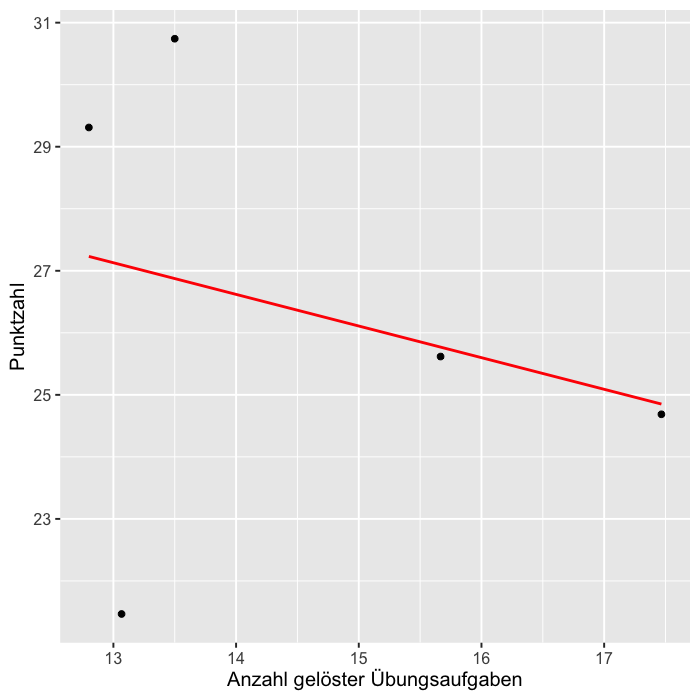
\includegraphics[width = 8cm, height = 8cm]{aggregation}
\caption{Zusammenhang zwischen der durchschnittlich gelösten Anzahl an Übungsaufgaben und der durschnittlich erreichten Punktzahl pro Klasse}
\label{fig:aggregiert}
\end{figure}

Die Analyse mittels Aggregation führt folglich nicht zu einem zufriedenstellenden Ergebnis und ist aufgrund der besprochenen Einschränkungen nicht geeignet, um Zusammenhänge auf Level-1 zu untersuchen.

\subsubsection{Disaggregation} \label{section:disaggregation}
Die zweite Möglichkeit um hierarchsiche Daten mit einem linearen Regressionsmodell zu untersuchen ist die Disaggregation. Wie bereits angedeutet werden bei der Disaggregation alle Level-2 Variablen auf Level-1 Einheiten verteilt. 

In unserem Beispiel werden also alle Schulkinder als voneinander unabhängige Datenpunkte in die Analyse miteinbezogen. Dazu werden jedem Schulkind aus derselben Klasse die gleichen Werte der Level-2 Variablen zugeschrieben. In Tabelle \ref{tab:beispiel_theorie} aus Abschnitt \ref{section:bsp_theorie} kann man dieses Vorgehen bei der Level-2 Variable \textit{Fenster} beobachten. Durch diese Disaggregation von Level-2 Variablen auf Level-1 Einheiten werden Datensätze künstlich vergrössert und mögliche Variabilität, die zwischen den Level-2 Variablen besteht, wird ignoriert \citep{SnijdersTomA.B2012Ma:a, woltman2012introduction}. Folglich wird die geteilte Varianz zwischen Level-1 Einheiten einer Gruppe nicht berücksichtigt und die Annahme, dass Fehler voneinander unabhängig sind, ist verletzt. Das führt dazu, dass die Effekte von Level-1 und Level-2 Variablen auf die abhängige Variable nicht voneinander getrennt werden können \citep{woltman2012introduction}. In unserem Beispiel würde das bedeuten, dass man den Einfluss der Anzahl gelöster Übungsaufgaben nicht vom Einfluss der Klasse trennen kann. Ein grundlegendes Problem der Disaggregation entsteht durch die Annahme von linearen Regressionsmodellen, dass einzelne Beobachtungen voneinander unabhängig sind \citep{woltman2012introduction}. Da bei hierarchischen Daten einzelne Beobachtungen voneinander Abhängig sind ist diese Annahme verletzt und Analysen basierend auf linearen Regressionsmodellen (z.B. Disaggregation) führen folglich zu ungenauen Ergebnissen \citep{andrew_data, SnijdersTomA.B2012Ma:a, woltman2012introduction}.

\begin{figure}[t!]
\centering
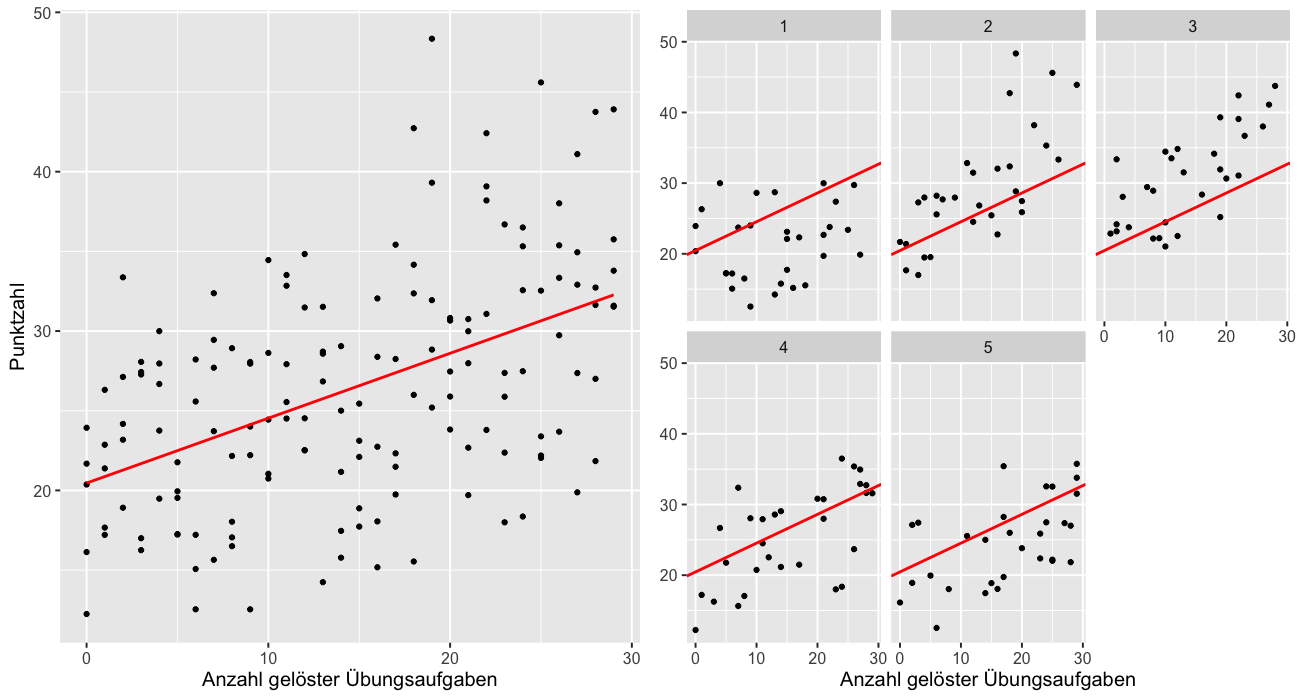
\includegraphics[width = \textwidth]{disaggregation_combined}
\caption{Zusammenhang zwischen der Anzahl gelöster Übungsaufgaben und erreichte Punktzahl mittels Disaggregation und Anwendung dieses Zusammenhangs auf jede der fünf Klassen}
\label{fig:disaggregation}
\end{figure}

Auf der linken Seite der Abbildung \ref{fig:disaggregation} befindet sich die Regressionsgerade, die durch ein lineares Regressionsmodell entsteht, wenn man mit einem disaggregierten Datensatz arbeitet. Anhand dieser Regressionsgerade besteht ein positiver Zusammenhang zwischen der Anzahl gelöster Übungsaufgaben und der erreichten Punktzahl in der Mathematikprüfung, so dass die erreichte Punktzahl mit steigender Anzahl an gelöster Übungsaufgaben zunimmt. Wie vorhin bereits erwähnt, wird in dieser Analyse aber nicht berücksichtigt, dass die Schulklasse selbst einen Effekt auf die erreichte Punktzahl haben kann. Dieser Effekt wird klar, wenn man die rechte Seite der Abbildung \ref{fig:disaggregation} betrachtet. Für jede der fünf Klassen wurde dieselbe Regressionsgerade, die aus dem disaggregierten Datensatz entsteht, über die Daten gelegt. Man kann relativ einfach erkennen, dass es gewisse Klassen gibt, bei denen mehr Schulkinder über oder unter der Regressionsgerade liegen. Des Weiteren kann man erkennen, dass es nicht optimal ist, wenn für alle Klassen dieselbe Steigung der Regressionsgerade verwendet wird. Betrachten wir beispielsweise die zweite Klasse, kann man erkennen, dass diese Schulkinder einen viel stärkeren Zusammenhang zwischen gelösten Übungsaufgaben und erreichter Punktzahl verzeichnen als die erste Klasse. Man könnte nun mit Hilfe einer Dummy-Kodierung den Einfluss von Klassen berücksichtigen, dazu müsste aber für jede Klasse einen zusätzlichen Parameter in das Modell aufgenommen werden. Bei unserem Datensatz mit nur fünf Klassen wäre das kein grosses Problem. Bei Datensätzen mit sehr vielen Klassen würde das bedeuten, dass ganz viele Parameter in das Modell aufgenommen werden müssten. Da es grundsätzlich erstrebenswert ist, möglichst sparsame Modelle zu bilden, ist auch dies keine optimale Lösung. 

Im letzten Abschnitt hat sich gezeigt, dass weder die Aggregation noch die Disaggregation der Daten zu zufriedenstellenden Ergebnissen führen, da sie massiven Einschränkungen unterliegen. Es erfordert folglich eine Erweiterung von LMs, die Zusammenhänge innerhalb und zwischen Level-2 Einheiten abbilden kann, ohne sich dabei auf eine Analyseeinheit festzulegen.

\subsection{Hierarchische Linearen Modelle}
In den letzten Abschnitten wurde angenommen, dass sich die Regressionskoeffizienten $\beta_0$ und $\beta_1$ feste Werte sind, die sich zwischen den Klassen nicht unterscheiden. In Abbildung \ref{fig:disaggregation} aus dem vorherigen Abschnitt konnte man aber erkennen, dass diese Annahme nicht in allen Fällen zu einem erwünschten Ergebnis führt. In unserem Beispiel gibt es offensichtlich Klassen, die eine über- oder unterdurchschnittliche Punktzahl erreichen. In HLMs können diese Unterschiede in den Regressionskoeffizienten zwischen den Klassen mittels zufälligen Effekten berücksichtigt werden. Unter einem zufälligen Effekt versteht man in diesem Kontext, dass die Koeffizienten der einzelnen Klassen zufällig voneinander abweichen. Die Varianz dieser zufälligen Abweichung wird von HLMs geschätzt und kann später dazu genutzt werden die einzelnen Regressionskoeffizienten der Klassen zu berechnen.

In den folgenden Abschnitten werden nun zwei Formen von HLMs besprochen, mit denen es möglich ist die Varianzen dieser Koeffizienten zu schätzen. Als erstes wird das \textit{Random Intercept} Modell vorgestellt. Dieses Modell geht davon aus, dass nur die Achsenabschnitte (\textit{Intercept}) der verschiedenen Klassen zufällig voneinander abweichen und die Steigung (\textit{Slope}) über alle Klassen konstant bleibt. Das zweite besprochenen Modell ist das \textit{Random Intercept and Slope} Modell. Bei diesem Modell wird angenommen, dass sich nicht nur die Achsenabschnitte der verschiedenen Klassen unterscheiden, sondern dass auch die Steigung zwischen den Klassen zufällig variiert.

\subsubsection{\textit{Random Intercept} Modell} \label{section:random_intercept_model}

Die einfachste Form eines \textit{Random Intercept} Modells ist ein Modell, das nur den Koeffizienten für den Achsenabschnitt $\beta_{0j}$ und das Residuum $\epsilon_i$ enthält. Dieses Modell wird wie folgt beschrieben:
\begin{equation}
\begin{split}	
\text{Level 1:} & \qquad y_{ij} 	= \beta_{0j} + \epsilon_{ij}\\
\text{Level 2:} & \qquad \beta_{0j} = \gamma_{00} + U_{0j}
\end{split}	
\end{equation} 
Bei dieser Darstellung handelt es sich um die hierarchische Notation der Gleichung, da die einzelnen Gleichungen gleich dem dazugehörigen Level zugeordnet werden. Dies wird klarer, wenn man es in Bezug zu unserem Beispiel betrachtet. Auf Level-1 befindet sich die Regressionsgleichung für die erreichte Punktzahl jedes einzelnen Schulkindes $i$ aus der Klasse $j$. Dabei kann man erkennen, dass der Regressionskoeffizient $\beta_{0j}$ von der Klasse $j$ abhängt und folglich für jede Klasse einen anderen Wert annimmt. Da die Klasse eine Level-2 Variable ist, befindet sich die Gleichung für $\beta_{0j}$ auf Level-2. Dabei ist $\gamma_{00}$ der Gesamtmittelwert und $U_{0j}$ die zufällige Abweichung der Klasse $j$ vom Gesamtmittelwert. Substituiert man die Gleichung von Level-2 in die Gleichung von Level-1, erhält man folgende Darstellung des \textit{Random Intercept} Modells:
\begin{equation}
\begin{split}
y_{ij} 	& = \beta_{0j} + \epsilon_{ij}\\
		& = \gamma_{00} + U_{0j} + \epsilon_{ij}
\end{split}
\end{equation}
Diese Gleichung entspricht dem leeren Modell aus Abschnitt \ref{section:icc}, anhand dessen man die IKK berechnet. Ähnlich wie bei der linearen Regression können diesem Modell weitere Variablen hinzugefügt werden, um die Varianz der erreichten Punktzahl des Schulkindes $i$ aus der Klasse $j$ zu erklären. In unserem Beispiel ergänzen wir das Modell mit nur einer weiteren Variable $x_{ij}$, die der Anzahl gelöster Übungsaufgaben entspricht:

\begin{equation} \label{eq:random_intercept_model}
\begin{split}	
 \text{Level 1:}  	\qquad 	y_{ij} 		& = \beta_{0j} + \beta_{1}x_{ij} + \epsilon_{ij}\\
 \text{Level 2:} 	\qquad 	\beta_{0j} 	& = \gamma_{00} + U_{0j}\\
 							\beta_{1} 	& = \gamma_{10}
\end{split}	
\end{equation} 
Da es sich hier um ein \textit{Random Intercept} Modell handelt, bleibt die Steigung für alle Klassen gleich. Dies kann man an der Gleichung des Koeffizienten $\beta_{1}$ erkennen, da es keine zufällige Abweichung in Abhängigkeit der Klasse $j$ von der Gesamtsteigung $\gamma_{10}$ gibt. Werden nun aus \eqref{eq:random_intercept_model} die beiden Gleichungen auf Level-2 in die Gleichung auf Level-1 eingesetzt, können wir das \textit{Random Intercept} Modell wieder mit nur einer Gleichung beschreiben:
\begin{equation}
\begin{split}
y_{ij} 	& = \beta_{0j} + \beta_{1}x_{ij} + \epsilon_{ij} \\
		& = \gamma_{00} + U_{0j} + \gamma_{10}x_{ij} + \epsilon_{ij} \\
		& = \gamma_{00} + \gamma_{10}x_{ij} + U_{0j} + \epsilon_{ij}
\end{split}
\end{equation}

In Abbildung \ref{fig:random_intercept} kann man nun die Geraden für jede einzelne Klasse erkennen. Die rote Gerade entspricht der linearen Regressionsgerade, die durch die Disaggregation entsteht und wird hier als Vergleichswert verwendet. Die schwarzen Geraden entsprechen den Geraden, die durch das \textit{Random Intercept} Modell geschätzt werden. Auf der linken Seite der Abbildung erkennt man relativ schnell, dass es bedeutende Unterschiede zwischen den Klassen gibt. Werden die Geraden für jede einzelne Klasse betrachtet, erhält man einen Überblick über das Leistungsniveau der verschiedenen Klassen. Beispielsweise kann man erkennen, dass die Klassen 1 und 5 eher tiefere und die Klassen 2 und 3 eher höhere Punktzahlen erreichen. Diese Unterschiede kommen durch die unterschiedliche Ausprägungen der zufälligen Abweichungen $U_{0j}$ zustande. 

\begin{figure}[ht!]
\centering
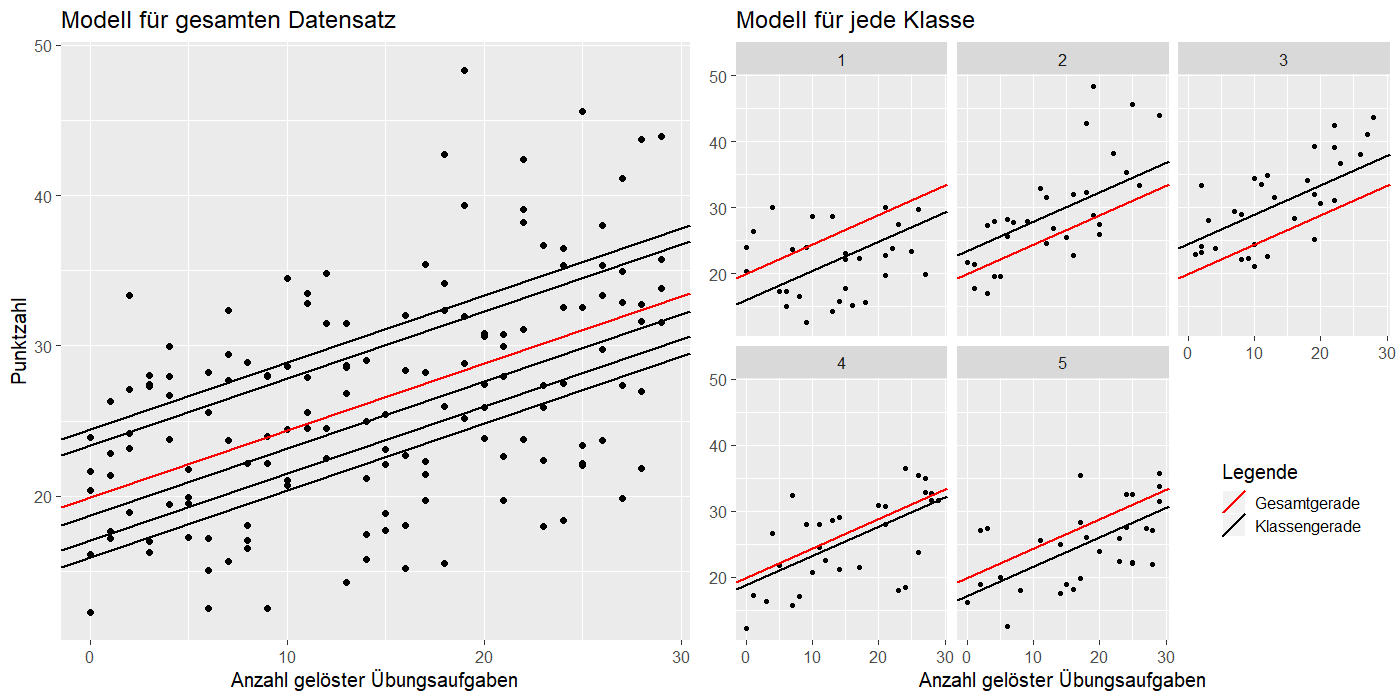
\includegraphics[width = \textwidth]{random_intercept}
\caption{Zusammenhang zwischen der Anzahl gelöster Übungsaufgaben und der erreichten Punktzahl mittels HLM im Vergleich zu einem LM (Disaggregation). Links: Geraden von LM und HLM im gesamten Datensatz. Rechts: Geraden von LM und HLM auf jede Klasse aufgeteilt.}
\label{fig:random_intercept}
\end{figure}

Da in HLMs nicht die zufällige Abweichung jeder einzelnen Klasse, sondern nur ihre Varianz geschätzt wird, müssen die zufällige Abweichung $U_{0j}$ und die daraus resultierenden Regressionskoeffizienten $\beta_{0j}$ zuerst berechnet werden. Diese Berechnung folgt einem in der psychologischen Testtheorie bekannten Prinzip, dem sogenannten \textit{shrinkage to the mean} \citep{SnijdersTomA.B2012Ma:a}. Dabei wird angenommen, dass sich Gruppenmittelwerte leicht in Richtung des Gesamtmittelwerts verschieben. Diese Annahme wird damit begründet, dass bei normalverteilten Daten Werte nahe am Gesamtmittelwert häufiger sind als extreme Werte. Da man bei HLMs davon aus geht, dass die zufällige Abweichung normal verteilt und im Mittel 0 ist, kann also das selbe Prinzip auch hier angewendet werden. In unserem Beispiel würde das bedeuten, dass der Mittelwert der erreichten Punktzahl der Klasse $j$ sich leicht in Richtung des Gesamtmittelwertes aller Beobachtungen $\gamma_{00}$ verschiebt. Wie stark aber dieser Mittelwert sich in Richtung des Gesamtmittelwertes verschiebt, wird durch eine Gewichtung dieser beider Mittelwerte festgelegt. Diese Gewichtung wird über die geschätzte Varianz der zufälligen Abweichung $U_{0j}$ berechnet. Ist die geschätzte Varianz der zufälligen Abweichung gross, dann werden Gruppenmittelwerte stärker gewichtet, ist die geschätzte Varianz klein, wird der Gesamtmittelwert stärker gewichtet. Die genauen Formeln und eine ausführlichere Beschreibung dieser Berechnung können in Snijders und Bosker \citeyearpar[][Abschnitt 4.8]{SnijdersTomA.B2012Ma:a} nachgeschlagen werden.

Für die Klasse 1 ergibt sich nun beispielsweise aus unserem \textit{Random Intercept} Modell eine berechnete gewichtete zufällige Abweichung von $U_{01} = -4.01$ und einen Schätzer für den Gesamtmittelwert $\gamma_{00} = 19.9$. Setzt man diese beiden Werte in die Gleichung aus \eqref{eq:random_intercept_model} erhält man den klassenspezifischen Achsenabschnitt $\beta_{01}$:
\begin{equation}
\beta_{01} = 19.9 - 4.01 = 15.89
\end{equation} 
Schulkinder der Klasse 1 erreichen bei $0$ gelösten Übungsaufgaben im Mittel eine Punktzahl von $15.89$. Für Klasse 2 lässt sich ihr Achsenabschnitt $\beta_{02}$ genau gleich bestimmen. Aus der klassenspezifischen Abweichung $U_{02} = 3.48$ und dem Gesamtmittelwert von $\gamma_{00} = 19.9$ ergibt sich ein Achsenabschnitt von $\beta_{02} = 23.38$. Schulkinder aus Klasse 2 erreichen bei 0 gelösten Übungsaufgaben im Mittel also eine höhere Punktzahl als Schulkinder aus Klasse 1. Diese Aussage stimmt ebenfalls mit den Geraden aus Abbildung \ref{fig:random_intercept} überein. Ebenfalls kann man beobachten, dass die Geraden des hierarchischen linearen Modells besser zu den Daten passen. Betrachtet man in Abbildung \ref{fig:random_intercept} auf der rechten Seite die Geraden der einzelnen Klassen kann man erkennen, dass die schwarzen Geraden des HLMs die Beobachtungen besser beschreiben, als die rote Gerade, die durch das LM geschätzt wird. Allerdings gibt es immer noch Schulkinder, die noch nicht optimal durch die Gerade des HLMs beschrieben werden. Bei der zweiten und dritten Klasse erreichten beispielsweise Schulkinder, die viele Übungen gelöst haben eine noch viel höhere Punktzahl als vom Modell angenommen wird. 

Anscheinend gibt es in unserem Datensatz Klassen, bei denen die Schulkinder einen stärkeren oder schwächeren Anstieg der erreichten Punktzahl bei steigender Anzahl gelöster Übungsaufgaben verzeichnen. Daraus könnte man nun folgern, dass sich nicht nur der Achsenabschnitt zwischen den Klassen unterscheidet, sondern auch die Steigung. Im folgenden Abschnitt wird nun das \textit{Random Intercept and Slope} Modell vorgestellt und überprüft, ob diese Form von HLM besser zu unseren Daten passt als ein \textit{Random Intercept} Modell.

\subsubsection{\textit{Random Intercept and Slope} Modell} \label{section:random_intercept_slope_model}

Im letzten Abschnitt wurde das \textit{Random Intercept} Modell besprochen und aufgezeigt, dass man durch die Hinzunahme von variierenden Achsenabschnitten eine bessere Passung zwischen dem Modell und den Daten erreicht. Um eine noch bessere Passung zu erreichen und genauere Vorhersagen zu treffen kann man nun nicht nur den Achsenabschnitt, sondern auch die Steigung variieren lassen. Dies führt zum \textit{Random Intercept and Slope} Modell, das sowohl Unterschiede in der abhängige Variablen zwischen den Klassen als auch Unterschiede im Einfluss der unabhängigen Variablen auf die abhängige Variable zwischen den Klassen berücksichtigt. Der Regressionskoeffizient $\beta_{1}$ aus dem \textit{Random Intercept} Modell \eqref{eq:random_intercept_model} ist nun spezifisch für jede Klasse $j$ und wird durch die zufällige Abweichung $U_{1j}$ erweitert. Dies führt zum folgenden Modell in der hierarchischen Notation:
\begin{equation} \label{eq:random_intercept_slope_model}
\begin{split}	
 \text{Level 1:}  \qquad y_{ij} & = \beta_{0j} + \beta_{1}x_{ij} + \epsilon_{ij}\\
 \text{Level 2:} \qquad \beta_{0j} & = \gamma_{00} + U_{0j}\\
 \beta_{1j} & = \gamma_{10} + U_{1j}
\end{split}	
\end{equation} 
Durch Einsetzen der Gleichungen aus Level-2 in die Gleichung aus Level-1, erhaltet man die folgende Gleichung des \textit{Random Intercept and Slope} Modells:
\begin{equation} \label{eq:flat_random_intercept_slope_model}
\begin{split}	
y_{ij} & = \beta_{0j} + \beta_{1}x_{ij} + \epsilon_{ij}\\
& = \gamma_{00} + U_{0j} + (\gamma_{10} + U_{1j})x_{ij} + \epsilon_{ij}\\
& = \gamma_{00} + \gamma_{10}x_{ij} + U_{0j} + U_{1j}x_{ij} + \epsilon_{ij}
\end{split}	
\end{equation} 
Dabei wurde die Gleichung so umgeformt, dass der erste Teil $\gamma_{00} + \gamma_{10}x_{ij}$ die jeweiligen geschätzten Parametern enthält, die sich nicht zwischen den Klassen verändern und wird folglich als fester Teil des Modells bezeichnet. Der zweite Teil der Gleichung mit $U_{0j} + U_{1j}x_{ij} + \epsilon_{ij}$ wird als zufälliger Teil bezeichnet, weil er alle zufällige Abweichungen und das Residuum enthält. Der Term $U_{1j}x_{ij}$ beschreibt den gruppenspezifischen Effekt, der die unabhängige Variable $x_{ij}$ auf die abhängige Variable hat. Bezogen auf unser Beispiel bedeutet dieser Term, wie stark und in welche Richtung sich die erreichte Punktzahl verändert in Abhängigkeit der Klassenzugehörigkeit und der Anzahl gelöster Übungen. 

\begin{figure}[t!]
\centering
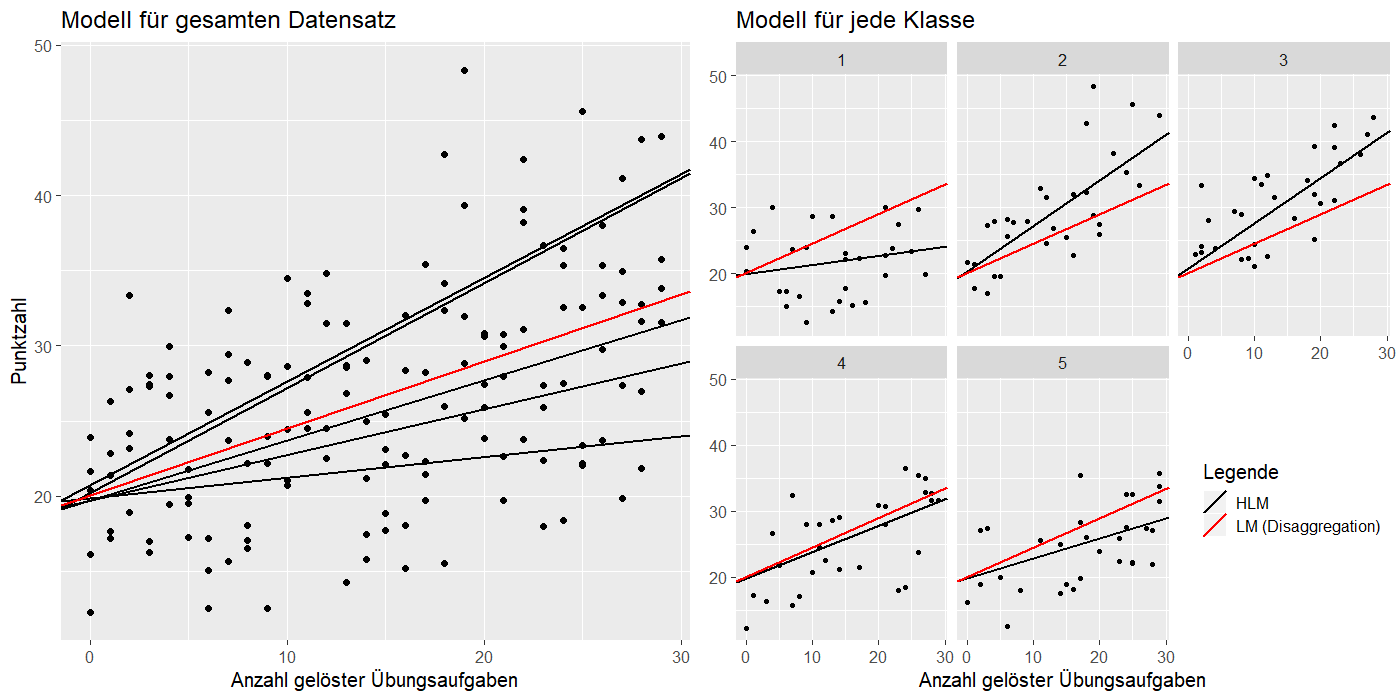
\includegraphics[width = \textwidth]{random_intercept_slope}
\caption{Zusammenhang zwischen der Anzahl gelöster Übungsaufgaben und der erreichten Punktzahl unter Berücksichtigung der Klassenzugehörigkeit und deren Effekt auf den Einfluss der Anzahl gelösten Übungsaufgaben. Links: Geraden von LM und HLM im gesamten Datensatz. Rechts: Geraden von LM und HLM auf jede Klasse aufgeteilt.}
\label{fig:random_intercept_slope}
\end{figure}

In Abbildung \ref{fig:random_intercept_slope} ist der Effekt der Klassenzugehörigkeit auf die Einfluss der Anzahl gelösten Übungsaufgaben einfach zu erkennen. Für gewisse Klassen nimmt die Zufallsvariable $U_{1j}$ eine positiven und für andere einen negativen Wert ein. Dies spiegelt sich wiederum in klassenspezifischen Steigungen $\beta_{1j}$ die höher oder tiefer als die Gesamtsteigung $\gamma_{10}$ ist. Wie bereits im \textit{Random Intercept} Modell werden auch im \textit{Random Intercept and Slope} Modell nur die Varianzen der zufälligen Abweichungen geschätzt und die Effektive zufällige Abweichung $U_{1j}$ muss ebenfalls berechnet werden. Diese Berechnung verläuft ebenfalls nach dem Prinzip von \textit{shrinkage to the mean}, wobei die Gruppensteigung leicht in Richtung der Gesamtsteigung verschoben wird.

Betrachten wir die Klasse 1 unseres Beispiels. Mit der Schätzung der Varianz der zufälligen Abweichung durch das \textit{Random Intercept and Slope} Modell lässt sich für diese Klasse die zufällige Abweichung von der Gesamtsteigung von $U_{11} = -0.24$ berechnen. Setzt man nun diesen Wert zusammen mit der Gesamtsteigung $\gamma_{10} = 0.45$ in die Gleichung für $\beta_{1j}$ aus \eqref{eq:random_intercept_slope_model} ein, erhält man die klassenspezifische Steigung $\beta_{11}$:
\begin{equation} \label{eq:beta1_example}	
\beta_{11} = 0.45 - 0.24 = 0.2
\end{equation} 
Für jede weitere gelöste Übungsaufgabe eines Schulkindes $i$ aus der Klasse 1 steigt also die erwartete Punktzahl im Mittel um $0.2$ Punkte an. Betrachten wir nun die Klasse 2 aus unserem Beispiel, schätzt unser Modell eine positive zufällige Abweichung $U_{12} = 0.2$ von der Gesamtsteigung. Wird dieser Wert wieder in die Gleichung für $\beta_{1j}$ aus \eqref{eq:random_intercept_slope_model} eingesetzt, erhalten wir einen klassenspezifische Steigung von $\beta_{12} = 0.65$. Diese Steigung ist nun grösser als die Gesamtsteigung $\gamma_{10} = 0.45$. Folglich nimmt die erreichte Punktzahl bei einer weiteren gelösten Übungsaufgabe eines Schulkindes $i$ aus der Klasse 1 im Mittel um $0.65$ zu. Schulkinder aus Klasse 2 verzeichnen also einen höheren Anstieg in der erreichten Punktzahl bei jeder weiteren gelösten Übungsaufgabe als Schulkinder aus Klasse 1. 

\begin{figure}[b!]
\centering
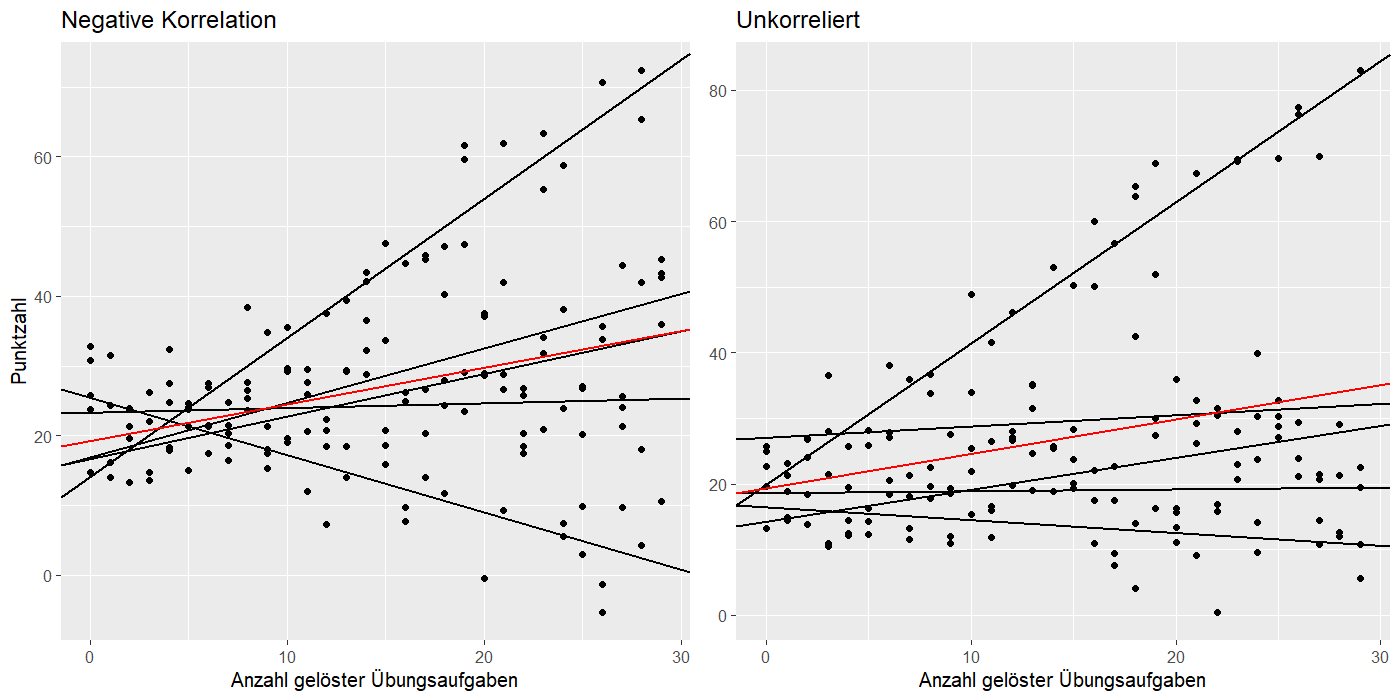
\includegraphics[width = \textwidth]{corr_s_i}
\caption{Darstellung einer negativen und nicht vorhandenen Korrelationen zwischen Achsenabschnitt und Steigung}
\label{fig:corr_s_i}
\end{figure}

In unserem Beispiel ist es so, dass je höher der klassenspezifische Achsenabschnitt ist, desto höher ist auch die klassenspezifische Steigung. Man spricht hier auch von einer positiven Korrelation zwischen Achsenabschnitt und Steigung. Diese beiden Koeffizienten müssen aber nicht zwingend positiv miteinander korreliert sein. Es gibt auch die Möglichkeit, dass diese Koeffizienten negativ korreliert oder sogar unkorreliert sind. In Abbildung \ref{fig:corr_s_i} kann man betrachten, wie die weiteren Korrelationen von Achsenabschnitt und Steigung sich auswirken. Auf der linken Seite der Abbildung ist eine negative Korrelation abgebildet. Bei einer negativen Korrelation nimmt die Steigung mit der Höhe des Achsenabschnittes ab. Sind die beiden Koeffizienten unkorreliert, bildet sich kein offensichtliches Muster zwischen der Höhe des Achsenabschnittes und der Steigung. Dieser Zusammenhang ist auf der rechten Seite der Abbildung zu sehen.

In diesem Abschnitt wurde das \textit{Random Intercept and Slope} Modell besprochen und es wurde gezeigt, dass ein Modell, bei dem sowohl der Achsenabschnitt als auch die Steigung zwischen den Klassen variiert, am besten zu unserem Datensatz passt. Im nächsten Abschnitt wird nun besprochen, wie diese Modelle durch die Hinzunahme von weiteren Prädiktoren in ihrer Fähigkeit, Variabilität in der abhängigen Variablen zu erklären, verbessert werden können.

\subsubsection{\textit{Intercept} und \textit{Slope} Variabilität} \label{section:variability}
Wie bei linearen Regressionsmodellen wird auch bei hierarchischen linearen Regressionsmodellen versucht die Variabilität einer bestimmten abhängigen Variablen zu erklären. Diese unerklärte Variabilität hängt in HLMs nicht nur von der Varianz des Residuums $\epsilon_{ij}$ ab, sondern auch von der Varianz der zufälligen Abweichung des Achsenabschnittes $U_{0j}$ und der Steigung $U_{1j}$ \citep{SnijdersTomA.B2012Ma:a}. Um nun unerklärte Variabilität in HLMs zu beschreiben, können die Varianzen all dieser Komponenten verringert werden. Um die Varianz des Residuums zu verringern können, wie bei der linearen Regression, weitere Level-1 Variablen in das Modell aufgenommen werden. Da die Varianzen der zufälligen Abweichungen nicht durch Unterschiede innerhalb der Gruppen sondern zwischen den Gruppen entstehen, können diese nicht durch das Hinzufügen von Level-1 Variablen reduziert werden, sondern erfordern das Hinzufügen von Level-2 Variablen. Snijders und Bosker \citeyearpar{SnijdersTomA.B2012Ma:a} erweitern hierfür die beiden Gleichungen für die Regressionskoeffizienten $\beta_{0j}$ und $\beta_{1j}$:
\begin{equation} \label{eq:variance}
\begin{split}	
 \text{Level 1:}  \qquad y_{ij} & = \beta_{0j} + \beta_{1}x_{ij} + \epsilon_{ij}\\
 \text{Level 2:} \qquad \beta_{0j} & = \gamma_{00} + \gamma_{01}z_{j} + U_{0j}\\
 \beta_{1j} & = \gamma_{10} + \gamma_{11}z_{j} + U_{1j}
\end{split}	
\end{equation}
Dabei ist $z_{j}$ eine Level-2 Variable, die sich zwischen den Gruppen unterscheidet. Auf unser Beispiel bezogen, könnte die Variable $z_{j}$ die Anzahl Fenster im Klassenzimmer sein. Durch das Hinzufügen dieser Level-2 Variablen werden die Regressionskoeffizienten selbst zu einer abhängigen Variablen eines Regressionmodells. Substituiert man die beiden Koeffizienten in die Level-1 Gleichung erhält man folgende Darstellung dieses HLMs:
\begin{equation} \label{eq:flat_variance}
\begin{split}	
y_{ij} & = \beta_{0j} + \beta_{1}x_{ij} + \epsilon_{ij}\\
& = \gamma_{00} + \gamma_{01}z_{j} + U_{0j} + (\gamma_{10} + \gamma_{11}z_{j} + U_{1j})x_{ij} + \epsilon_{ij}\\
& = \gamma_{00} + \gamma_{01}z_{j} + U_{0j} + \gamma_{10}x_{ij} + \gamma_{11}z_{j}x_{ij} + U_{1j}x_{ij} + \epsilon_{ij}\\
& = \gamma_{00} + \gamma_{01}z_{j} + \gamma_{10}x_{ij} + \gamma_{11}z_{j}x_{ij} + U_{0j} + U_{1j}x_{ij} + \epsilon_{ij}\\
\end{split}	
\end{equation} 
Auch wenn es in der hierarchischen Notation einfacher zu erkennen ist, welche Varianz genau durch die Hinzunahme dieser Level-2 Variable verringert wird, erkennt man in dieser Notation einen weiteren wichtigen Zusammenhang. Der Term $\gamma_{11}z_{j}x_{ij}$ beschreibt eine besondere Interaktion zwischen einer Level-1 und einer Level-2 Variable und wird, wie bereits in der Einleitung kurz erwähnt, als \textit{Cross-Level} Interaktion bezeichnet. Da diese \textit{Cross-Level} Interaktion durch das Hinzufügen einer Level-2 Variable als Prädiktor in der Gleichung des Steigungskoeffizienten entsteht, ist diese Interaktion vor allem wichtig, um unerklärte Varianz in der Steigung zu erklären. In unserem Beispiel würde diese \textit{Cross-Level} Interaktion also durch die Interaktion zwischen der Anzahl gelösten Übungsaufgaben und der Anzahl Fenster im Klassenzimmer beschrieben werden. Die Anzahl der Fenster erklären also einen Anteil der Variabilität in der Steigung zwischen den Klassen bezüglich des Effekts der Anzahl gelösten Übungsaufgaben auf die erreichte Punktzahl.

In den letzten Abschnitten wurden zwei verschiedene HLMs besprochen und das Prinzip ihrer Anwendung diskutiert. Es ist dabei zu berücksichtigen, dass hier nur die Grundlagen zu den HLMs behandelt wurden. Für eine weitere Vertiefung dieses Themas wird auf die gängige Literatur zur Multilevel Analyse mittels HLMs verwiesen \citep{andrew_data, raudenbush2002hierarchical, SnijdersTomA.B2012Ma:a, twisk_2006}. Im anschliessenden Abschnitt wird die praktische Anwendung von HLMs in R mit dem Paket \texttt{lme4} \citep{batesetal2015lme4} besprochen.

\subsection{Anwendung von HLMs in R} \label{section:ml_in_R}
Das Konzept von hierarchischen linearen Modellen wurde in den letzten Abschnitten ausführlich besprochen. In den nächsten Abschnitten wird vor allem die Anwendung dieser Modelle behandelt. Dabei wird der Fokus auf die Programmiersprache R gelegt und dessen Zusatzpaket \texttt{lme4} \citep{batesetal2015lme4}, das neben weiteren Paketen die Analyse mittels HLMs ermöglicht. Dabei wird davon ausgegangen, dass die Grundlagen dieser Programmiersprache verstanden wurden. Zuerst werden allgemeine Informationen und die Syntax von \texttt{lme4} besprochen. Anschliessend wird Schritt für Schritt ein HLM erstellt und der \texttt{summary()}-Output wird interpretiert. Hierbei wird aufgezeigt, wie HLMs aufgebaut und miteinander verglichen werden, um das geeignetste Modell zu identifizieren. Am Ende dieses Abschnittes werden Effektstärkemasse besprochen, die bei der Auswertung und Berichterstattung von HLMs wichtig sind.  

\subsubsection{Informationen und Syntax von \texttt{lme4}}
Mit dem Paket \texttt{lme4} lassen sich verschiedenste Formen von hierarchischen Modellen schätzen und analysieren. Dabei werden wir uns hier hauptsächlich auf die Funktion \texttt{lmer()} beschränken. Diese Funktion wird verwendet, um hierarchische lineare Modelle zu schätzen und dessen Syntax ist relativ ähnlich mit der Syntax des Befehls für die Berechnung normaler linearer Modelle \texttt{lm()}. Sie ist wie folgt aufgebaut:

\begin{knitrout}
\definecolor{shadecolor}{rgb}{0.969, 0.969, 0.969}\color{fgcolor}\begin{kframe}
\begin{alltt}
\hlkwd{lmer}\hlstd{(formula, data, REML, ...)}
\end{alltt}
\end{kframe}
\end{knitrout}

Dabei wird in \texttt{formula} die gewünschte Formel des Modells eingegeben, bei \texttt{data} wird der Datensatz festgelegt anhand das Modell geschätzt werden soll und bei \texttt{REML} wird durch einen logischen Operator (\textit{TRUE} oder \textit{FALSE}) eingestellt, ob das Modell mit \textit{Restricted Maximum Likelihood} (REML) oder mit \textit{Maximum Likelihood} (ML) geschätzt werden soll. Beide dieser Methoden erzeugen eine \textit{Log-Likelihood} aus der die \textit{Deviance} berechnet werden kann. Die \textit{Deviance} gibt die relative Passung eines Modells zu den Daten an und kann folglich genutzt werden, um zwei Modelle miteinander zu vergleichen \citep{SnijdersTomA.B2012Ma:a}. Allerdings unterscheidet sich die Bedeutung der \textit{Deviance} zwischen ML und REML. Unter ML gibt die \textit{Deviance} an, wie gut die geschätzten Regressionskoeffizienten und die geschätzte Varianz zu den Daten passt. Wohingegen die \textit{Deviance} unter REML nur angibt, wie gut die geschätzten Varianzen zu den Daten passen. Dieses Argument ist also vor allem dann wichtig, wenn man Modelle vergleichen möchte. Dabei sollte ML für den Vergleich von festen Effekten und REML für den Vergleich von zufälligen Effekten verwendet werden \citep{PEUGH201085}. Die drei Punkte in der Funktion stehen für weitere Argumente, die in \texttt{lmer()} eingegeben werden können. Diese Argumente werden aber hier nicht weiter behandelt, da sie für eine erweiterte Anwendung verwendet werden und den Rahmen dieser Arbeit sprengen würden\footnote{Mit dem Befehl \texttt{?lmer} kann die gesamte Dokumentation von \texttt{lmer()} angezeigt werden.}

Der folgende Code zeigt exemplarische Darstellung, wie eine Formel in \texttt{lmer()} eingegeben wird:

\singlespacing
\begin{knitrout}
\definecolor{shadecolor}{rgb}{0.969, 0.969, 0.969}\color{fgcolor}\begin{kframe}
\begin{alltt}
\hlkwd{lmer}(Abhängige Variable ~ Feste Effekte + (Zufällige Effekte | Gruppe),...)
\end{alltt}
\end{kframe}
\end{knitrout}
\setstretch{1.5}

Bis zum Term innerhalb der Klammer ist die Syntax von \texttt{lmer()} genau die gleiche wie bei \texttt{lm()}. Dabei wird auf zuerst die zu erklärende Variable aufgeführt und anschliessend alle Variablen, die als feste Effekte in das Modell aufgenommen werden sollen. Innerhalb der Klammern können nun die zufälligen Effekte und die variierende Gruppe festgelegt werden. Dabei gibt es viele Möglichkeiten, wie zufällige Effekte und Gruppen in das Modell aufgenommen werden können. Beispielsweise können mehrere Gruppen definiert werden für die der Achsenabschnitt variiert oder dass sich nur die Steigung zwischen den Gruppen unterscheidet. Da es in diesem Abschnitt nur um die grundlegende Anwendung von \texttt{lmer()} geht, werden diese Möglichkeiten hier nicht behandelt. Eine Ausführliche Beschreibung der Anwendung von \texttt{lmer()} und dem gesamten Paket von \texttt{lme4} kann in Bates et al. \citeyearpar{batesetal2015lme4} nachgeschlagen werden. In Tabelle \ref{tab:lmersyntax} ist nun die Syntax für die drei Möglichkeiten aufgeführt, die auch in diesem Abschnitt besprochen sind.
\begin{table}[ht] 
\centering
\begin{threeparttable}
\caption{Auswahl der möglichen Syntax für \texttt{lmer()} nach Bates et al. \citeyearpar{batesetal2015lme4}. Der Buchstabe \textit{g} beschreibt hier den Gruppenfaktor und \textit{x} die weiteren zufälligen Effekte.}
\begin{tabular}{lll}
 	\toprule
	Formel & Alternative & Bedeutung\\ 
  	\midrule
	(1 $|$ g)	& - 		& Zufälliger Achsenabschnitt \\
	(x $|$ g) 	& (1 + x $|$ g)	& Korrelierter Achsenabschnitt und Steigung \\
	(x $||$ g) & (1 $|$ g) + (0 + x $|$ g)	& Unkorrelierter Achsenabschnitt und Steigung\\
  	\bottomrule
\end{tabular}
\label{tab:lmersyntax}
\end{threeparttable}
\end{table}

\subsubsection{Aufbau und Vergleich von HLMs} \label{section:hlm_r}
\singlespacing

\setstretch{1.5}
Wir gelangen nun zur Analyse unseres Beispieldatensatzes. Bevor wir mit der Analyse starten können ist es wichtig, dass wir das Level unserer Forschungsfrage klar definieren. In unserem Fall möchten wir herausfinden, wie genau sich die Prüfungsleistung von Schulkindern mit der Anzahl gelöster Übungsaufgaben unter Berücksichtigung der Klassenzugehörigkeit verändert. Das bedeutet, dass sich unsere abhängige Variable auf Level-1 befindet. Ebenfalls sollte berücksichtigt werden, dass es zu Interaktionen zwischen Level-1 und Level-2 variablen kommen kann.

Als Erstes berechnen wir die IKK, um den Einfluss der Klassenzugehörigkeit zu quantifizieren. Wie bereits im Abschnitt \ref{section:icc} besprochen, lässt sich die IKK aus den Varianzen des leeren Modells berechnen, das hier noch einmal kurz aufgeführt ist:

\begin{equation}
\begin{split}	
 \text{Level 1:}  \qquad y_{ij} & = \beta_{0j} + \epsilon_{ij}\\
 \text{Level 2:} \qquad \beta_{0j} & = \gamma_{00} + U_{0j}\\
\end{split}	
\end{equation} 
Dieses Modell wird wie folgt in R mittels der Funktion \texttt{lmer()} geschätzt:

\singlespacing
\begin{knitrout}
\definecolor{shadecolor}{rgb}{0.969, 0.969, 0.969}\color{fgcolor}\begin{kframe}
\begin{alltt}
\hlstd{m_leer} \hlkwb{<-} \hlkwd{lmer}\hlstd{(punktzahl} \hlopt{~} \hlstd{(}\hlnum{1} \hlopt{|} \hlstd{klasse),} \hlkwc{data} \hlstd{= beispiel_data,}
    \hlkwc{REML} \hlstd{=} \hlnum{TRUE}\hlstd{)}

\hlkwd{print}\hlstd{(}\hlkwd{VarCorr}\hlstd{(m_leer),} \hlkwc{comp} \hlstd{=} \hlstr{"Variance"}\hlstd{)}
\end{alltt}
\begin{verbatim}
##  Groups   Name        Variance
##  klasse   (Intercept) 12.3    
##  Residual             44.0
\end{verbatim}
\end{kframe}
\end{knitrout}
\setstretch{1.5}

Aus diesem Modell können nun die Varianzen für den Achsenabschnitt $\tau^2 = 12.33$ und das Residuum $\sigma^2 = 44$ ausgelesen und in die Formel \eqref{eq:icc} eingesetzt werden. Daraus ergibt sich die bereits in Abschnitt \ref{section:icc} berechnete IKK von $\rho_I = 0.22$. Folglich werden 22\% der Variabilität in der erreichten Punktzahl durch die Klassenzugehörigkeit erklärt.

Wir können nun damit anfangen unser leeres Modell mit weitere Prädiktoren aufzubauen, um mehr Variabilität in der abhängigen Variablen zu erklären. In unserem Beispiel fügen wir die Anzahl gelöster Übungsaufgaben als festen Effekt dem Modell hinzu. Natürlich könnten hier noch weitere feste Effekte hinzugefügt werden, damit das Beispiel aber übersichtlich bleibt, ist das Modell hier auf einen festen Effekt beschränkt:

\begin{equation}
\begin{split}	
 \text{Level 1:}  \qquad y_{ij} & = \beta_{0j} + \beta_{1} \cdot \text{uebungen}_{ij} + \epsilon_{ij}\\
 \text{Level 2:} \qquad \beta_{0j} & = \gamma_{00} + U_{0j}\\
 \beta_{1} & = \gamma_{10}\\
\end{split}	
\end{equation} 
In der oberen Gleichung kann man erkennen, dass es sich hier um ein einfaches \textit{Random Intercept} Modell handelt, da bei $\beta_{1}$ keine zufällige Abweichung hinzugefügt wurde. Um nun ein \textit{Random Intercept} Modell in R zu schätzen wird der Funktion die Variable wie folgt hinzugefügt:

\singlespacing
\begin{knitrout}
\definecolor{shadecolor}{rgb}{0.969, 0.969, 0.969}\color{fgcolor}\begin{kframe}
\begin{alltt}
\hlstd{m_intercept} \hlkwb{<-} \hlkwd{lmer}\hlstd{(punktzahl} \hlopt{~} \hlstd{uebung} \hlopt{+} \hlstd{(}\hlnum{1} \hlopt{|} \hlstd{klasse),}
        \hlkwc{data} \hlstd{= beispiel_data,} \hlkwc{REML} \hlstd{=} \hlnum{TRUE}\hlstd{)}
\end{alltt}
\end{kframe}
\end{knitrout}
\setstretch{1.5}

Dabei ist zu beachten, dass der Term innerhalb der Klammern der Vorgabe aus Tabelle \ref{tab:lmersyntax} entspricht, um ein \textit{Random Intercept} Modell zu schätzen. Wir haben nun also ein leeres Modell und ein \textit{Random Intercept} Modell mit einem Prädiktor. Möchten wir jetzt überprüfen, ob unser grösseres Modell besser zu den Daten passt als das leere Modell und mehr Varianz aufklärt, kann man wie beim Vergleich von normalen LMs mit dem Befehl \texttt{anova()} die Modelle miteinander Vergleichen. 

\singlespacing
\begin{knitrout}
\definecolor{shadecolor}{rgb}{0.969, 0.969, 0.969}\color{fgcolor}\begin{kframe}
\begin{alltt}
\hlkwd{anova}\hlstd{(m_leer, m_intercept,} \hlkwc{method} \hlstd{=} \hlstr{"LRT"}\hlstd{)}
\end{alltt}


{\ttfamily\noindent\itshape\color{messagecolor}{\#\# refitting model(s) with ML (instead of REML)}}\begin{verbatim}
## Data: beispiel_data
## Models:
## m_leer: punktzahl ~ (1 | klasse)
## m_intercept: punktzahl ~ uebung + (1 | klasse)
##             Df  AIC  BIC logLik deviance Chisq Chi Df
## m_leer       3 1009 1018   -502     1003             
## m_intercept  4  952  964   -472      944  59.1      1
##             Pr(>Chisq)    
## m_leer                    
## m_intercept    1.5e-14 ***
## ---
## Signif. codes:  
## 0 '***' 0.001 '**' 0.01 '*' 0.05 '.' 0.1 ' ' 1
\end{verbatim}
\end{kframe}
\end{knitrout}
\setstretch{1.5}

Da sich zwischen diesen beiden Modellen nur feste Effekte unterscheiden, sie aber mittels REML geschätzt wurden, schätzt \texttt{anova()} die beiden Modelle nochmals neu mit der ML Methode. Ausserdem ist zu Beachten, dass beim Vergleich von zwei HLMs nicht wie bei normalen LMs ein \textit{F} Test sondern ein \textit{Likelihood Ratio Test} verwendet wird \citep{PEUGH201085,SnijdersTomA.B2012Ma:a}. Dieser Test verwendet die Differenz der \textit{Deviance} als Prüfgrösse einer $\chi^2$-Verteilung. Bei einem signifikanten Ergebnis passt das komplexere Modell mit mehr Parametern besser zu den Daten und bei einem nicht-signifikaten Test wird das einfachere Modell beibehalten, da es bereits genügend gut zu den Daten passt.

Im oberen Output ist also zu entnehmen, dass unser \textit{Random Intercept} Modell auf einem Signifikanzniveau von 5\% besser zu den Daten passt als das leere Modell. Wir möchten nun zusätzlich ein \textit{Random Intercept and Slope} Modell schätzen. Entsprechend des Abschnittes \ref{section:random_intercept_slope_model} wird der Gleichung von $\beta_{1j}$ eine zufällige Abweichung von der mittleren Steigung hinzugefügt: 
\begin{equation} 
\begin{split}	
 \text{Level 1:}  \qquad y_{ij} & = \beta_{0j} + \beta_{1} \cdot \text{uebungen}_{ij} + \epsilon_{ij}\\
 \text{Level 2:} \qquad \beta_{0j} & = \gamma_{00} + U_{0j}\\
 \beta_{j1} & = \gamma_{10 }+ U_{1j}\\
\end{split}	
\end{equation} 
Diese zufällige Abweichung der Steigung wird nun auch in der Formel in R hinzugefügt:

\singlespacing
\begin{knitrout}
\definecolor{shadecolor}{rgb}{0.969, 0.969, 0.969}\color{fgcolor}\begin{kframe}
\begin{alltt}
\hlstd{m_uncorr} \hlkwb{<-} \hlkwd{lmer}\hlstd{(punktzahl} \hlopt{~} \hlstd{uebung} \hlopt{+} \hlstd{(uebung} \hlopt{||} \hlstd{klasse),}
        \hlkwc{data} \hlstd{= beispiel_data,} \hlkwc{REML} \hlstd{=} \hlnum{TRUE}\hlstd{)}
\end{alltt}
\end{kframe}
\end{knitrout}
\setstretch{1.5}

Dabei ist zu beachten, dass hier keine Korrelation zwischen Achsenabschnitt und Steigung angenommen wird, da man erst einmal einfach überprüfen möchte, ob überhaupt ein Modell mit einer variierenden Steigung besser zu den Daten passt als eines ohne. Werden nun zwei Modelle miteinander Verglichen, die sich nur in ihren zufälligen Effekten unterscheiden, können beide Modelle mittels REML geschätzt werden \citep{PEUGH201085}. Um sicherzustellen, dass \texttt{anova()} die Modelle nicht nochmals neu mit ML schätzt, kann ihr das Argument \texttt{refit = FALSE} hinzugefügt werden. Im folgenden Output ist das Ergebnis des \textit{Likelihood Ratio Tests} aufgeführt:

\singlespacing
\begin{knitrout}
\definecolor{shadecolor}{rgb}{0.969, 0.969, 0.969}\color{fgcolor}\begin{kframe}
\begin{alltt}
\hlkwd{anova}\hlstd{(m_intercept, m_uncorr,} \hlkwc{method} \hlstd{=} \hlstr{"LRT"}\hlstd{,} \hlkwc{refit} \hlstd{=} \hlnum{FALSE}\hlstd{)}
\end{alltt}
\begin{verbatim}
## Data: beispiel_data
## Models:
## m_intercept: punktzahl ~ uebung + (1 | klasse)
## m_uncorr: punktzahl ~ uebung + ((1 | klasse) + (0 + uebung | klasse))
##             Df AIC BIC logLik deviance Chisq Chi Df
## m_intercept  4 953 965   -473      945             
## m_uncorr     5 945 960   -467      935  10.7      1
##             Pr(>Chisq)   
## m_intercept              
## m_uncorr        0.0011 **
## ---
## Signif. codes:  
## 0 '***' 0.001 '**' 0.01 '*' 0.05 '.' 0.1 ' ' 1
\end{verbatim}
\end{kframe}
\end{knitrout}
\setstretch{1.5}

Der \textit{Likelihood Ratio Test} kommt also zum Ergebnis, dass ein Modell, das eine zufällige Abweichung der Steigung zulässt bei einem Signifikanzniveau von 5\% besser zu den Daten passt. Vergleicht man die beiden Abbildungen \ref{fig:random_intercept} und \ref{fig:random_intercept_slope} scheint dieses Ergebnis des \textit{Likelihood Ratio Test} glaubhaft zu sein. Wir möchten nun auch noch herausfinden, ob ein Modell, das eine Korrelation zwischen Achsenabschnitt und Steigung annimmt, besser ist als unser unkorreliertes Modell. Dazu wird gemäss der Tabelle \ref{tab:lmersyntax} ein weiteres Modell geschätzt und mit unserem unkorrelierten Modell verglichen.

\singlespacing
\begin{knitrout}
\definecolor{shadecolor}{rgb}{0.969, 0.969, 0.969}\color{fgcolor}\begin{kframe}
\begin{alltt}
\hlstd{m_corr} \hlkwb{<-} \hlkwd{lmer}\hlstd{(punktzahl} \hlopt{~} \hlstd{uebung} \hlopt{+} \hlstd{(uebung} \hlopt{|} \hlstd{klasse),} \hlkwc{data} \hlstd{= beispiel_data,}
    \hlkwc{REML} \hlstd{=} \hlnum{TRUE}\hlstd{)}

\hlkwd{anova}\hlstd{(m_uncorr, m_corr,} \hlkwc{method} \hlstd{=} \hlstr{"LRT"}\hlstd{,} \hlkwc{refit} \hlstd{=} \hlnum{FALSE}\hlstd{)}
\end{alltt}
\begin{verbatim}
## Data: beispiel_data
## Models:
## m_uncorr: punktzahl ~ uebung + ((1 | klasse) + (0 + uebung | klasse))
## m_corr: punktzahl ~ uebung + (uebung | klasse)
##          Df AIC BIC logLik deviance Chisq Chi Df Pr(>Chisq)
## m_uncorr  5 945 960   -467      935                        
## m_corr    6 946 964   -467      934  1.19      1       0.27
\end{verbatim}
\end{kframe}
\end{knitrout}
\setstretch{1.5}

Das Ergebnis des \textit{Likelihood Ratio Tests} zeigt, dass bei einem Signifikanzniveau von 5\% das Modell mit einer Korrelation nicht besser zu den Daten passt. Folglich wird in diesem Fall ein \textit{Random Intercept and Slope} Modell beibehalten, das von keiner Korrelation zwischen Achsenabschnitt und Steigung ausgeht.

Bis jetzt haben wir uns nur mit Level-1 Variablen oder der zufälligen Abweichung beschäftigt. Möchten wir dem Modell die Anzahl Fenster im Klassenzimmer als Level-2 Variable hinzufügen, kann man diese Variable mit einer \textit{Cross-Level} Interaktion oder ohne hinzufügen. Ebenfalls ist zu beachten, dass Level-2 Variablen in einem hierarchischen linearen Modell mit zwei Level nur mit festen Effekten hinzugefügt werden können. Da es in einem zwei Level Modell nicht noch ein drittes höheres Level gibt, in dem eine Level-2 Variable noch zwischen Level-3 Einheiten variieren könnte. In der Formel würde das Hinzufügen einer Level-2 Variable ohne \textit{Cross-Level} Interaktion wie folgt aussehen:
\begin{equation} 
\begin{split}	
 \text{Level 1:}  \qquad y_{ij} & = \beta_{0j} + \beta_{1} \cdot \text{uebungen}_{ij} + \epsilon_{ij}\\
 \text{Level 2:} \qquad \beta_{0j} & = \gamma_{00} + \gamma_{01} \cdot \text{fenster}_{j} + U_{0j}\\
 \beta_{j1} & = \gamma_{1j} + U_{1j}\\
\end{split}	
\end{equation} 

In R ist das Hinzufügen von Level-2 Variablen relativ einfach, da eine Level-2 Variable in unserem Fall nur als fester Effekt hinzugefügt werden kann, wird sie einfach in die Gleichung vor dem Term in der Klammer eingefügt. Möchte man die Level-2 Variable als \textit{Cross-Level} Interaktion hinzufügen, kann für das $+$ einfach ein $*$ eingesetzt werden. In diesem Modell wird aber die Level-2 Variable einfach als fester Effekt hinzugefügt.

\singlespacing
\begin{knitrout}
\definecolor{shadecolor}{rgb}{0.969, 0.969, 0.969}\color{fgcolor}\begin{kframe}
\begin{alltt}
\hlstd{m_fix_lvl2} \hlkwb{<-} \hlkwd{lmer}\hlstd{(punktzahl} \hlopt{~} \hlstd{uebung} \hlopt{+} \hlstd{fenster} \hlopt{+} \hlstd{(uebung} \hlopt{||} \hlstd{klasse),}
        \hlkwc{data} \hlstd{= beispiel_data,} \hlkwc{REML} \hlstd{=} \hlnum{TRUE}\hlstd{)}
\end{alltt}
\end{kframe}
\end{knitrout}
\setstretch{1.5}

Nachdem das neue Modell mit der Level-2 Variable geschätzt wurde, kann es wieder mit dem sparsameren Modell \texttt{m\_uncorr} verglichen werden. Da sich zwischen den beiden Modellen wieder nur die festen Effekte unterscheiden, werden von \texttt{anova()} die Modelle wieder neu mit ML geschätzt. Im folgenden Output ist zu erkennen, dass das komplexere Modell mit einer Level-2 Variable auf einem Signifikanzniveau von 5\% nicht besser zu den Daten passt als unser vorheriges Modell. Die Level-2 Variable Anzahl Fenster kann also aus dem Modell ausgeschlossen werden.

\singlespacing
\begin{knitrout}
\definecolor{shadecolor}{rgb}{0.969, 0.969, 0.969}\color{fgcolor}\begin{kframe}
\begin{alltt}
\hlkwd{anova}\hlstd{(m_uncorr, m_fix_lvl2,} \hlkwc{method} \hlstd{=} \hlstr{"LRT"}\hlstd{)}
\end{alltt}


{\ttfamily\noindent\itshape\color{messagecolor}{\#\# refitting model(s) with ML (instead of REML)}}\begin{verbatim}
## Data: beispiel_data
## Models:
## m_uncorr: punktzahl ~ uebung + ((1 | klasse) + (0 + uebung | klasse))
## m_fix_lvl2: punktzahl ~ uebung + fenster + ((1 | klasse) + (0 + uebung | 
## m_fix_lvl2:     klasse))
##            Df AIC BIC logLik deviance Chisq Chi Df
## m_uncorr    5 944 959   -467      934             
## m_fix_lvl2  6 942 960   -465      930  3.37      1
##            Pr(>Chisq)  
## m_uncorr               
## m_fix_lvl2      0.066 .
## ---
## Signif. codes:  
## 0 '***' 0.001 '**' 0.01 '*' 0.05 '.' 0.1 ' ' 1
\end{verbatim}
\end{kframe}
\end{knitrout}
\setstretch{1.5}

\subsubsection{Interpretation eines HLMs}
Im letzten Abschnitt wurde ein HLM von Grund auf aufgebaut, mit dem Versucht wurde den Zusammenhang zwischen der Anzahl gelösten Übungsaufgaben und der erreichten Punktzahl in einer Mathematikprüfung unter Berücksichtigung der Klassenzugehörigkeit zu erklären. Dabei ergab sich nach mehreren Modellvergleichen, dass ein \textit{Random Intercept and Slope} Modell mit unkorrelierten Achsenabschnitten und Steigungen unter Berücksichtigung der Modellkomplexität am besten zu unseren Daten passt.

Nun geht es darum dieses Modell zu interpretieren. Als erstes kann man mit dem \texttt{summary()} Befehl eine Zusammenfassung ausgeben, die man für eine erste Interpretation unseres Modells verwenden kann. Der \texttt{summary()}-Output des HLMs ähnelt dem eines LMs. Dabei werden aber die zufälligen und die festen Effekte getrennt aufgeführt. 

\singlespacing
\begin{knitrout}
\definecolor{shadecolor}{rgb}{0.969, 0.969, 0.969}\color{fgcolor}\begin{kframe}
\begin{alltt}
\hlkwd{summary}\hlstd{(m_uncorr)}
\end{alltt}
\begin{verbatim}
## Linear mixed model fit by REML ['lmerMod']
## Formula: 
## punktzahl ~ uebung + ((1 | klasse) + (0 + uebung | klasse))
##    Data: beispiel_data
## 
## REML criterion at convergence: 935
## 
## Scaled residuals: 
##     Min      1Q  Median      3Q     Max 
## -2.1103 -0.8016  0.0542  0.7212  2.8707 
## 
## Random effects:
##  Groups   Name        Variance Std.Dev.
##  klasse   (Intercept)  0.8560  0.925   
##  klasse.1 uebung       0.0646  0.254   
##  Residual             26.8972  5.186   
## Number of obs: 150, groups:  klasse, 5
## 
## Fixed effects:
##             Estimate Std. Error t value
## (Intercept)   20.036      0.933   21.47
## uebung         0.446      0.124    3.59
## 
## Correlation of Fixed Effects:
##        (Intr)
## uebung -0.312
\end{verbatim}
\end{kframe}
\end{knitrout}
\setstretch{1.5}


Bei den zufälligen Effekten werden für den Achsenabschnitt als auch für die Steigung die geschätzte Varianzen und die Standardabweichungen. Da in unserem Modell keine Korrelationen geschätzt wurden, wird diese hier nicht angezeigt. Ebenfalls werden direkt unterhalb der zufälligen Effekte aufgeführt wie gross die verwendete Stichprobe war und wie viele Gruppen für die Schätzung verwendet wurden. In unserem Fall waren das 150 Schulkinder, verteilt auf 5 Klassen. Der Abschnitt zu den festen Effekten ähnelt stark dem Output eines LMs und lässt sich auch dementsprechend interpretieren. Es werden hier aber keine $p$-Werte angezeigt, da man sich in der Forschung noch nicht einig darüber ist, wie genau die Anzahl der Freiheitsgrade geschätzt werden soll \citep{PEUGH201085,SnijdersTomA.B2012Ma:a}\footnote{Möchte man $p$-Werte anzeigen lassen, kann man das mit dem Paket \texttt{lmerTEST} \citep{lmertest}.}. 


Bei der Interpretation ist es von Vorteil die Standardabweichung zu verwenden, da diese nicht wie die Varianz quadriert ist und somit der Masseinheit, in unserem Beispiel der Punktzahl, entspricht. Eine Interpretation des Achsenabschnittes unter Berücksichtigung der zufälligen Effekte würde dann wie folgt lauten: 
\begin{quote}
Die erreichte Punktzahl in der Mathematikprüfung von 95\% der Schulkinder liegt zwischen  $20.04 \pm 1.96 \cdot 0.93$ Punkten, wenn keine einzige Übungsaufgabe gelöst wurde.
\end{quote}
Und für die Steigung:
\begin{quote}
Die Zunahme der Punktzahl liegt bei 95\% der Schulkinder zwischen $0.45 \pm 1.96 \cdot 0.25$ Punkten pro gelöste Übungsaufgabe.
\end{quote}
Dabei ist 0.93 die Standardabweichung des Achsenabschnittes und 0.25 die Standardabweichung der Steigung. Die Zahl 1.96 ist eine Approximation für das 97.5te Perzentil einer Standardnormalverteilung und wird hier verwendet, um den Bereich zu berechnen, der 95\% aller Beobachtungen enthält. 

\subsubsection{Effektstärkemasse von HLMs}
Effektstärkemasse gibt es für normale lineare Regressionsmodelle einige, wie zum Beispiel das Bestimmtheitsmass $R^2$ oder das Cohen's $d$. Bei HLMs werden Effektstärkemasse in globale und lokale Effektstärkemasse getrennt \citep{PEUGH201085}. Dabei gibt es bei den globalen Effektstärkemasse mehrere Formen zur Berechnung eines Bestimmtheitsmasses $R^2$. Allerdings herrscht hier keinen Konsens über die bestmögliche Berechnungsform \citep{raudenbush2002hierarchical,SnijdersTomA.B2012Ma:a}. In diesem Abschnitt wird die Berechnung des Bestimmtheitsmasses $R^2$ von Snijders und Bosker \citeyearpar{SnijdersTomA.B2012Ma:a} behandelt. Bei dieser Berechnungsform wird davon ausgegangen, dass bei HLMs auf mehreren Levels die proportional erklärte Varianz berechnet werden kann. Ausgehend von unserem Beispiel mit zwei Levels kann man proportional erklärte Varianz auf Stufe des Individuums und auf Stufe der Gruppe berechnen. Snijders und Bosker \citeyearpar{SnijdersTomA.B2012Ma:a} geben an, dass vor allem die proportionale erklärte Varianz des Individuums von praktischer Relevanz ist und wird durch $R_{1}^2$ gekennzeichnet. Die Berechnung von $R_{1}^2$ erfolgt mit folgender Formel:
\begin{equation} \label{eq:r_square}
\begin{split}	
 R_{1}^2 & = 1 - \dfrac{\text{Gesamtvarianz des Modells mit Prädiktoren}}{\text{Gesamtvarianz des leeren Modells}} \\
 & \\
 & = 1 - \dfrac{\sigma^2 + \tau_{0}^2}{\sigma_{leer}^2 + \tau_{0leer}^2}
\end{split}	
\end{equation}
Dabei ist $\sigma^2$ die jeweilige Varianz des Residuums und $\tau_{0}^2$ die Varianz des Achsenabschnittes des jeweiligen Modelles. Da in der Berechnung von $R_{1}^2$ die Varianz der Steigung nicht berücksichtigt wird, kann dieses Effektstärkemass nur für \textit{Random Intercept} Modelle berechnet werden. Die Berechnung von $R_{1}^2$ für \textit{Random Intercept and Slope} Modellen ist viel aufwändiger, da in diesem Fall auch noch die Varianz der Steigung miteinbezogen werden muss. Gemäss Snijders und Bosker liegen aber die $R_{1}^2$ Werte von einem \textit{Random Intercept} Modell normalerweise sehr nahe an den $R_{1}^2$ Werten eines \textit{Random Intercept and Slope} Modells, wenn in beiden Modellen die selben festen Effekten vorhanden sind \citep{SnijdersTomA.B2012Ma:a}. Daher reicht es in dem meisten Fällen völlig aus, die einfache Berechnung von $R_{1}^2$ für \textit{Random Intercept} Modelle zu verwenden.

Für unser Beispiel würde das nun bedeuten, dass die Varianzen aus dem \textit{Random Intercept} Modell verwendet werden können, um ein $R_{1}^2$ zu berechnen, dass nahe am $R_{1}^2$ des \textit{Random Intercept and Slope} Modells \texttt{m\_uncorr} liegt. Das \textit{Random Intercept} Modell wurde bereits in Abschnitt \ref{section:hlm_r} geschätzt und ist hier zur Übersicht noch einmal aufgeführt:

\singlespacing
\begin{knitrout}
\definecolor{shadecolor}{rgb}{0.969, 0.969, 0.969}\color{fgcolor}\begin{kframe}
\begin{alltt}
\hlstd{m_intercept} \hlkwb{<-} \hlkwd{lmer}\hlstd{(punktzahl} \hlopt{~} \hlstd{uebung} \hlopt{+} \hlstd{(}\hlnum{1} \hlopt{|} \hlstd{klasse),}
                \hlkwc{data} \hlstd{= beispiel_data,} \hlkwc{REML} \hlstd{=} \hlnum{TRUE}\hlstd{)}

\hlkwd{print}\hlstd{(}\hlkwd{VarCorr}\hlstd{(m_intercept),} \hlkwc{comp} \hlstd{=} \hlstr{"Variance"}\hlstd{)}
\end{alltt}
\begin{verbatim}
##  Groups   Name        Variance
##  klasse   (Intercept) 15.5    
##  Residual             29.3
\end{verbatim}
\end{kframe}
\end{knitrout}
\setstretch{1.5}



\setstretch{1.5}

Die Varianzen des leeren Modells können im Abschnitt \ref{section:hlm_r} entnommen und mit den Varianzen für das \textit{Random Intercept} Modell aus dem oberen Output in die Formel eingesetzt werden:
\begin{equation} 
\begin{split}	
 R_{1}^2 & = 1 - \dfrac{29.29 + 15.46}{44 + 12.33} = 0.21
\end{split}	
\end{equation}
Folglich kann man nun die Aussage treffen, dass das \textit{Random Intercept} Modell \texttt{m\_intercept} 21\% der Varianz in der erreichten Punktzahl von Schulkindern erklärt. Gemäss Snijders und Bosker \citeyearpar{SnijdersTomA.B2012Ma:a} entspricht dieser Wert also ungefähr der Varianzaufklärung unseres \textit{Random Intercept and Slope} Modells \texttt{m\_uncorr}. 

Es gibt aber auch Situationen in denen man genau wissen möchte, wie viel Varianz durch die Hinzunahme eines bestimmten Prädiktors im Modell erklärt wird. Dies kann man mit der proportionalen Reduktion der Varianz (PRV) erklären, die als eines der lokale Effektstärkemasse von hierarchischen linearen Modellen gilt \citep{PEUGH201085, woltman2012introduction}. Wie bereits in früheren Abschnitten erläutert, wird bei HLMs die Varianz des Residuums sowohl auch die Varianzen des Achsenabschnittes und der Steigung geschätzt. In Abschnitt \ref{section:variability} wurde angesprochen, dass durch die Hinzunahme von weitere Prädiktoren diese Varianzen gezielt verringert werden können. Durch die Berechnung der PRV, kann nun die Reduktion in der Varianz bei allen drei geschätzten Varianzen des HLMs quantifiziert werden. Die Berechnung erfolgt für alle Varianzen mit der selben Formel:
\begin{equation} \label{eq:prv}
\begin{split}	
 PRV = \dfrac{Var_{0} - Var_{1}}{Var_{0}}
\end{split}	
\end{equation}
Dabei ist $Var_{0}$ die Varianz des Modells, das den gewünschten Prädiktor nicht enthält und $Var_{1}$ des Modells, das den Prädiktor enthält. Gehen wir nun ganz an den Anfang unserer Analyse zurück und überprüfen, wie viel Varianz des Residuums im Vergleich zum leeren Modell durch die Hinzunahme der Anzahl gelösten Übungsaufgaben als Prädiktor reduziert wird. Dazu wurden folgend die Varianzkomponenten des leeren Modells und des ersten \textit{Random Intercept} Modells ausgegeben. 

\singlespacing
\begin{knitrout}
\definecolor{shadecolor}{rgb}{0.969, 0.969, 0.969}\color{fgcolor}\begin{kframe}
\begin{alltt}
\hlstd{m_leer} \hlkwb{<-} \hlkwd{lmer}\hlstd{(punktzahl} \hlopt{~} \hlstd{(}\hlnum{1} \hlopt{|} \hlstd{klasse),}
                \hlkwc{data} \hlstd{= beispiel_data,} \hlkwc{REML} \hlstd{=} \hlnum{TRUE}\hlstd{)}

\hlkwd{print}\hlstd{(}\hlkwd{VarCorr}\hlstd{(m_leer),} \hlkwc{comp} \hlstd{=} \hlstr{"Variance"}\hlstd{)}
\end{alltt}
\begin{verbatim}
##  Groups   Name        Variance
##  klasse   (Intercept) 12.3    
##  Residual             44.0
\end{verbatim}
\begin{alltt}
\hlstd{m_intercept} \hlkwb{<-} \hlkwd{lmer}\hlstd{(punktzahl} \hlopt{~} \hlstd{uebung} \hlopt{+} \hlstd{(}\hlnum{1} \hlopt{|} \hlstd{klasse),}
                \hlkwc{data} \hlstd{= beispiel_data,} \hlkwc{REML} \hlstd{=} \hlnum{TRUE}\hlstd{)}

\hlkwd{print}\hlstd{(}\hlkwd{VarCorr}\hlstd{(m_intercept),} \hlkwc{comp} \hlstd{=} \hlstr{"Variance"}\hlstd{)}
\end{alltt}
\begin{verbatim}
##  Groups   Name        Variance
##  klasse   (Intercept) 15.5    
##  Residual             29.3
\end{verbatim}
\end{kframe}
\end{knitrout}


\setstretch{1.5}

Die Varianz der Residuen des leeren Modells beträgt $\sigma_{0}^2 = 44$ und die Varianz der Residuen des \textit{Random Intercept} Modells $\sigma_{1}^2 = 29.29$. Fügen wir diese beiden Werte in die Formel \eqref{eq:prv} ein erhalten wir die proportionale Reduktion der Varianz des Residuums:
\begin{equation} 
\begin{split}	
 PRV_{R} = \dfrac{44 - 29.29}{44} = 0.33
\end{split}	
\end{equation}
Daraus kann nun geschlossen werden, dass durch die Hinzunahme der Anzahl gelösten Übungsaufgaben als Prädiktor für die erreichte Punktzahl in der Mathematikprüfung eine Reduktion der Residualvarianz von 33\% erreicht wird. Da wir in unserem Modell nur eine Level-1 Variable als festen Effekt hinzugefügt haben, kann keine weitere PRV für den Achsenabschnitt und der Steigung berechnet werden. Möchte man die Varianzen dieser beiden Koeffiziente reduzieren, müssen wie bereits in Abschnitt \ref{section:variability} besprochen Level-2 Variablen in das Modell aufgenommen werden. Erst dann kann auch die proportionale Reduktion der Varianz mit der oberen Formel berechnet werden.

Wir haben nun zwei Effektstärkemasse von HLMs besprochen. Zum einen das globale Effektstärkemass $R_{1}^2$, das dazu genutzt werden kann, um die gesamte erklärte Varianz eines Modells zu beschreiben. Dieses Effektstärkemass ist vor allem dann nützlich, wenn man aussagen darüber treffen möchte, wie gut ein Modell die vorhandenen Daten beschreibt. Möchte man aber wissen wie viel Varianz durch einzelne bestimmte Prädiktoren erklärt werden, kann man mit dem lokalen Effektstärkemass der PRV für jeden Prädiktor die aufgeklärte Varianz berechnen. Zusätzlich ist die PRV auch nützlich, um die Varianzen zu identifizieren, die am meisten durch den gewählten Prädiktor reduziert werden.

Im letzten Abschnitt wurde anhand eines einfachen Beispiels aufgezeigt, wie man eine ein HLM in R aufbaut und analysiert. Das Ziel dieses Abschnittes war es in erster Linie zu zeigen, wie mit dem Paket \texttt{lme4} arbeitet und welche Möglichkeiten es gibt, um hierarchische Daten in R zu analysieren.

\section{Simulationsstudie zur Multilevel Analyse}
Der Einfluss von hierarchischen Datenstrukturen auf die Analyse wurden konzeptionell in den letzten Abschnitten diskutiert und vorgestellt. Im folgenden Abschnitt geht es nun, um die wissenschaftliche Replikation und Überprüfung dieses Einflusses. Dabei wird vor allem der Fokus auf die Unterschiede zwischen der Analyse mittels normalen linearen Modellen (LM) und hierarchischen linearen Modellen (HLM) gelegt. Um diese beide Methoden zu vergleichen, wird eine Simulationsstudie durchgeführt. Anschliessend an die Simulationsstudie wird eine Shiny App \citep{shiny} vorgestellt, die im Laufe dieser Arbeit programmiert wurde und mit der es Nutzern möglich ist, zum einen das Konzept der HLM zu verstehen und zum anderen werden die Ergebnisse dieser Simulationsstudie interaktiv für die Nutzer dargestellt.

\subsection{Herleitung der Forschungsfrage}
In der Einleitung wurde bereits erwähnt, dass in der psychologischen Forschung hierarchische Datenstrukturen keine Seltenheit sind und in Tabelle \ref{tab:beispiele_levels} wurden einige Beispiele für solche hierarchischen Daten genannt \citep{raudenbush2002hierarchical,SnijdersTomA.B2012Ma:a,woltman2012introduction}. Allerdings ist es oft so, dass sich Forschende dieser Datenstruktur oder den Möglichkeiten von HLMs nicht bewusst sind \citep{mcneish2014analyzing}. Dies kann dazu führen, dass diese hierarchischen Daten mittels normalen LMs anstelle von HLMs analysiert werden. Simulationsstudien haben aber gezeigt, dass dies nicht zwingend ein Problem darstellen muss \citep{mcneish2014analyzing, mundfrom2002monte}. In diesen Simulationsstudien wurden systematisch Datensätze mit unterschiedlichen IKKs generiert, um den Einfluss der Gruppenzugehörigkeit zu variieren. Basierend auf diesen Datensätzen wurden von LMs und HLMs die Regressionskoeffizienten geschätzt und miteinander verglichen. Diese Vergleiche ergaben, dass sowohl HLMs als auch normale LMs die Grösse des Regressionskoeffizienten relativ genau schätzen konnten, unabhängig davon wie gross der Einfluss der Gruppenzugehörigkeit auf die abhängige Variable war  \citep{mcneish2014analyzing, mundfrom2002monte}. Diese Ergebnisse deuten also darauf hin, dass die Schätzung der Grösse des Effekts einer Intervention oder des Achsenabschnitts bei beiden Methoden relativ nahe am Populationsmittelwert liegt.

Allerdings interessiert man sich in der Forschung oft nicht nur für die Grösse des Effekts, sondern auch ob dieser einen signifikanten Einfluss hat. Um zu überprüfen, ob eine Intervention auch effektiv einen Einfluss auf die Ausprägung der abhängige Variable hat, werden üblicherweise \textit{t} Tests durchgeführt \citep{SnijdersTomA.B2012Ma:a}. Die Prüfgrösse des \textit{t} Tests wird über das Verhältnis zwischen dem geschätzten Regressionskoeffizienten und dessen Standardfehlers bestimmt. Wird beispielsweise ein Standardfehler zu klein geschätzt, steigt die Prüfgrösse an und die Rate mit der die Nullhypothese abgelehnt wird, nimmt zu. Wird der Standardfehler zu gross geschätzt, verkleinert sich die Prüfgrösse und die Rate mit der die Alternativhypothese abgelehnt wird, nimmt zu. Folglich führt eine Unterschätzung des Standardfehlers zu einer erhöhten Fehler Typ 1 Rate und eine Überschätzung zu einer erhöhten Fehler Typ 2 Rate und somit zu einer geringeren Power \citep{SnijdersTomA.B2012Ma:a}. Unter Power wird die Wahrscheinlichkeit verstanden, einen Effekt zu finden, wenn dieser auch effektiv in der Population vorhanden ist \citep{scherbaumferreter2009powersample}. Daher ist eine genaue Schätzung des Standardfehlers umso wichtiger, da dieser massgeblich zur Power des Tests beiträgt. Da der Standardfehler in einem direkten Zusammenhang mit der Stichprobengrösse steht und grössere Stichproben zu kleineren Standardfehlern führen, ist die Wahl der Stichprobengrösse ein entscheidender Faktor \citep{james2013introduction, SnijdersTomA.B2012Ma:a}. Bei hierarchischen Daten sind Beobachtungen aus derselben Gruppe ähnlicher zueinander als zu anderen Beobachtungen aus anderen Gruppen. Folglich verkleinert sich die effektive Stichprobengrösse \citep{raudenbush2002hierarchical}. Wie stark sich die effektive Stichprobengrösse in einem hierarchischen Datensatz mit zwei Levels verkleinert, hängt zum einen von der Gruppengrösse und der Grösse des Einflusses der Gruppenzugehörigkeit ab. Dies kann mit dem sogenannten \textit{Design Effect} quantifiziert werden und wird mit der folgenden Formel berechnet \citep{raudenbush2002hierarchical,SnijdersTomA.B2012Ma:a}:
\begin{equation}
\textit{Design Effect} = 1 + (n - 1) \rho_I
\end{equation}
Dabei wird angenommen, dass die Gruppengrösse $n$ bei allen Gruppen gleich gross und $\rho_I$ die IKK ist. Mit zunehmender IKK und Gruppengrösse erhöt sich folglich der \textit{Design Effect}. Zum Beispiel würde das bei einer IKK von $\rho_I = 0.5$ und einer Stichprobe von $N = 100$ Schulklassen mit jeweils $n = 10$ Schulkindern pro Schulklasse zu einem \textit{Design Effect} von 5.5 führen. Obwohl hier Beobachtungen von 1000 Schulkindern erfasst wurden, erhaltet man aufgrund der hierarchsichen Datenstruktur nur eine effektive Stichprobe von $M_{\text{effektiv}} = 182$:
\begin{equation}
M_{\text{effektiv}} = \frac{Nn}{\textit{Design Effect}} = \frac{1000}{5.5} = 182
\end{equation}
Ein normales LM würde in diesem Fall mit einer Stichprobengrösse von 1000 arbeiten, um den Standardfehler zu berechnen und nicht mit der effektiven Stichprobengrösse. Bei HLMs wird diese hierarchische Struktur bei der Berechnung des Standardfehlers berücksichtigt \citep{snijdersbosker1993SEcalc}. Da ein HLM die hierarchische Struktur berücksichtigt und ein LM nicht, müssten diese beide Modelle zu unterschiedlichen Standardfehlern und dementsprechend auch zu verschiedenen Prüfgrössen für den \textit{t} Test gelangen. 

Diese Erkenntnis bestätigte sich schon in mehreren Simulationsstudien und theoretischen Artikeln \citep[z.B.][]{guo2005groupeddatahlm, krullmackinnon2010mediation, mcneish2014analyzing, MOERBEEK2003341}. Dabei ergab sich in diesen Artikeln, dass der Standardfehler von LMs in Abhängigkeit des Studiendesigns und der Analyseart unter- oder überschätzt wird. Beispielsweise fanden Krull und MacKinnon \citeyearpar{krullmackinnon2010mediation}, dass die Standardfehler eines Mediationseffekts konstant von LMs unterschätzt wurden und folglich zu einer erhöhten Fehler Typ 1 Rate führten. Diese Unterschätzung stieg mit zunehmender IKK sogar noch weiter an \citep{krullmackinnon2010mediation}. McNeish \citeyearpar{mcneish2014analyzing} fand ebenfalls, dass der Standardfehler des Achsenabschnittes von LMs konstant unterschätzt wurde und bei steigender IKK die Unterschätzung zunahm. Allerdings wurde der Standardfehler nicht immer unterschätzt. Moerbeek et al. \citeyearpar{MOERBEEK2003341} konnten in ihrem Artikel an einem simulierten und an einem realen Datensatz zeigen, dass der Standardfehler eines Interventionseffekts je nach Studiendesign von LMs unter- oder überschätzt wurde. Wird eine Intervention auf Level-1 durchgeführt, d.h. die zufällige Zuweisung zu einer Interventions- oder Kontrollgruppe geschieht auf der Individualebene, können Standardfehler durch LM überschätzt werden und folglich zu einer niedrigeren Power führen \citep{MOERBEEK2003341}. Wird eine Intervention auf Level-2 durchgeführt und die zufällige Zuweisung zu einer Interventions- oder Kontrollgruppe findet auf der Gruppenebene statt, führte dies wieder zu einer Unterschätzung des Standardfehlers \citep{MOERBEEK2003341}. In all diesen Studien konnte allerdings gezeigt werden, dass HLMs nicht diesen Limitationen unterlagen und den Standardfehler durchgehend genau geschätzt haben.

Neben der Prüfgrösse ist auch die Anzahl an Freiheitsgrade relevant, um die Signifikanz eines Effekts mittels \textit{t} Test zu überprüfen. Während bei normalen LMs die Anzahl Freiheitsgrade durch $N - p - 1$ bestimmt wird, wobei $N$ die Stichprobengrösse und $p$ die Anzahl Parameter im Modell sind, ist die Berechnung der Freiheitsgrade bei HLMs nicht eindeutig geklärt und ein aktueller Forschungsgegenstand \citep{mcneish2014analyzing,raudenbush2002hierarchical,SnijdersTomA.B2012Ma:a}.

Wie man in den vorherigen Studien erkennen kann, gibt es viele Faktoren, die einen Einfluss auf die Grösse des Standardfehlers haben. Um diese Einflüsse zu untersuchen werden zwei Simulationsstudien durchgeführt. Das Ziel der ersten Simulationsstudie ist es Teile dieser vorherigen Studien zu replizieren. Dabei wird der Einfluss von der IKK und des Studiendesigns auf die Schätzgenauigkeit der Regressionskoeffizienten und des Standardfehlers von LMs und HLMs untersucht. Gemäss der vorherigen Studien von Krull und MacKinnon \citeyearpar{krullmackinnon2010mediation} und McNeish \citeyearpar{mcneish2014analyzing} wird erwartet, dass bei zunehmender IKK die Schätzgenauigkeit von LMs abnimmt, bei HLMs aber konstant bleibt. Ausserdem wird davon ausgegangen, dass der Standardfehler des Interventionseffekts bei einer Intervention auf Level-1 gemäss Moerbeek et al. \citeyearpar{MOERBEEK2003341} überschätzt wird, sofern keine Interaktion zwischen Intervention und Gruppenzugehörigkeit angenommen wird. Ebenfalls wird angenommen, dass bei einer Intervention auf Level-2 der Standardfehler des Interventionseffekts durch LMs wieder unterschätzt wird. In beiden Simulationsdesigns wird gemäss Moerbeek et al. \citeyearpar{MOERBEEK2003341} erwartet, dass HLMs eine konstant genaue Schätzung der Standardfehler vorweisen.

Wie bereits erläutert führen zu klein geschätzte Standardfehler zu einer erhöhten Fehler Typ 1 Rate. Diese erhöhte Fehler Typ 1 Rate resultiert folglich in auffällig kleinen $p$-Werten \citep{raudenbush2002hierarchical, SnijdersTomA.B2012Ma:a}. In einer Studie von Guo \citeyearpar{guo2005groupeddatahlm} wurde gezeigt, dass ein $p$-Wert eines Effekts der basierend auf auf einem LM berechnet wurde, halb so gross war, wie der $p$-Wert eines HLMs. Dies führte dazu, dass ein LM diesen Effekt als signifikant und ein HLM als nicht signifikant identifizierten \citep{guo2005groupeddatahlm}. Aber auch das Gegenteil ist ein Problem. Werden Standardfehler Überschätzt erhöht sich die Fehler Typ 2 Rate und die Power verkleinert sich. In seinem Artikel erwähnte Guo ebenfalls, dass vor allem bei der Suche nach kleinen Effektstärken oder bei kleineren Stichproben die Gefahr besteht, dass ein LM zu fehlerhaften Ergebnissen gelangt \citep{guo2005groupeddatahlm}. Diese Schätzungenauigkeiten können also zu fehlerhaften Schlussfolgerungen führen und es sollte folglich im Interesse jedes Forschenden sein, diese zu vermeiden. 

Folglich wird in einer zweiten kleineren Simulationsstudie untersucht, wie sich die Fehlerraten und die Power dieser beiden Analysemethoden bei einer kleineren Stichprobe und in Abhängigkeit der IKK verhält. Wie in der ersten Simulationsstudie, werden auch in der zweiten Simulationsstudie die beiden Interventionsdesigns von Moerbeek et al. \citeyearpar{MOERBEEK2003341} untersucht. Dabei werden bei einem Interventionsdesign auf Level-1 grundsätzlich eine höhere Power erwartet, da in diesem Design der Effekt der Gruppenzugehörigkeit vom Effekt der Intervention getrennt werden kann \citep{moerbeek2000design}. Ebenfalls wird erwartet, dass die Power von LM bei einer Intervention auf Level-1 mit zunehmender IKK abnimmt, da angenommen wird, dass es zunehmend zu einer Überschätzung des Standardfehlers kommt und dieser zu einer erhöhten Fehler Typ 2 Rate führt. Die Power eines HLMs sollte aber über alle IKK Bedingungen konstant bleiben, da gemäss den besprochenen Studien ein HLM auch bei zunehmender IKK den Standardfehler genau schätzt \citep{mcneish2014analyzing}. Bei einer Intervention auf Level-2 werden aufgrund des Interventionsdesigns grundsätzlich bei beiden Analysemethoden keine hohe Power erwartet \citep{moerbeek2000design}. Allerdings wird erwartet, dass die Power von LMs höher als die Power von HLMs ist, da gemäss Moerbeek et al. \citeyearpar{MOERBEEK2003341} in dieser Situation die Standardfehler von LMs zunehmend unterschätzt werden und eine erhöhte Fehler Typ 1 Rate diese vermeintlich höhere Power verursacht.

\subsection{Simulationsdesign} \label{section:sim_design}
Um diese Annahmen zu überprüfen werden in beiden Simulationsstudien Daten basierend auf denselben zwei Designs von Moerbeek et al. \citeyearpar{MOERBEEK2003341} generiert. Beim ersten Design handelt es sich um eine Intervention auf Level des Schulkindes und die Daten werden anhand der folgenden Gleichung generiert:
\begin{equation} 
\begin{split}
\text{Design 1:}\\	
 \text{Level 1:}  \qquad y_{ij} & = \beta_{0j} + \beta_{1}x_{ij} + \epsilon_{ij}\\
 \text{Level 2:} \qquad \beta_{0j} & = \gamma_{00} + U_{0j}\\
 \beta_{1} & = \gamma_{10}\\
 \end{split}	
\end{equation} 
Dabei ist $\epsilon_{ij}$ das Residuum des $i$-ten Schulkindes aus der $j$-ten Klasse. Die Variable $x_{ij}$ gibt an, ob sich das Schulkind $i$ aus der Klasse $j$ in der Interventions- oder Kontrollgruppe befindet. Der Koeffizient $\beta_{0j}$ beschreibt den Achsenabschnitt, der wiederum durch den Gesamtmittelwert $\gamma_{00}$ und der zufälligen Abweichung $U_{0j}$ der Klasse $j$ beschrieben wird. Der Koeffizient $\beta_{j1}$ wird nur durch die Gesamtsteigung $\gamma_{1j}$ beschrieben. Folglich wird keine klassenspezifische Abweichung der Steigung in der Studie simuliert.

Das zweite Design berücksichtigt Interventionen auf Stufe der Klassen. Dabei werden die Daten nach der folgenden Gleichung generiert:

\begin{equation} 
\begin{split}
 \text{Design 2:}\\
  \text{Level 1:}  \qquad y_{ij} & = \beta_{0j} + \epsilon_{ij}\\
 \text{Level 2:} \qquad \beta_{0j} & = \gamma_{00} + \gamma_{01}z_{j} + U_{0j}\\
\end{split}	
\end{equation} 
Wieder beschreibt $\epsilon_{ij}$ das Residuum des $i$-ten Schulkindes aus der $j$-ten Klasse. Der Achsenabschnitt $\beta_{0j}$ wird durch den Gesamtmittelwert $\gamma_{00}$, der Gesamtsteigung $\gamma_{01}$, der Variable $z_{j}$ und der klassenspezifischen zufälligen Abweichung $U_{0j}$ beschrieben. Die Variable $z_{j}$ gibt an, zu welcher Interventionsgruppe die $j$-te Klasse gehört. Da in diesem Design die Intervention auf Stufe der Klasse durchgeführt wird, handelt es sich bei der Intervention um eine Level-2 Variable und wird typischerweise mit $z_{j}$ und nicht mit $x_{j}$ bezeichnet. Es wird in beiden Designs angenommen, dass die zufälligen Effekte $\epsilon_{ij}$ und $U_{0j}$ voneinander unabhängig sind und einer Normalverteilung folgen. Ebenfalls wird angenommen, dass diese zufällige Effekte einen Mittelwert von Null und eine Varianz von $\sigma^{2}_{e}$, resp. $\tau^{2}_{0}$ aufweisen.

Gewisse Parameter werden in beiden Simulationsstudien nicht manipuliert. Für diese Parameter wurden dieselben Werte von Moerbeek et al. \citeyearpar{MOERBEEK2003341} und McNeish \citeyearpar{mcneish2014analyzing} verwendet. Die Zuweisung zur Interventionsgruppe wurde für die Variablen $x_{ij}$ und $z_{j}$ durch die Werte -1 und 1 festgelegt. Dabei steht -1 für die Kontrollgruppe und 1 für die Interventionsgruppe. Der Gesamtmittelwert der Population wurde in beiden Designs auf $\gamma_{00}$ = 2.34 festgelegt. Die Gesamtsteigung der Population wurde ebenfalls in der gesamten Simulationsstudie mit $\gamma_{10}$ = 0.12 für die Gesamtsteigung der Level-1 Variable und $\gamma_{01}$ = 0.12 für die Gesamtsteigung der Level-2 Variable festgehalten. Für das Residuum wurde eine Varianz von $\sigma^{2}_{e}$ = 1.72 und ein Erwartungswert von 0 verwendet. Diese Werte stammen alle aus der Simulation von Moerbeek et al. \citeyearpar{MOERBEEK2003341}, die ihre Werte auf einem Teildatensatz des \textit{Television School and Family Smoking Prevention and Cessation Projekt (TVSFP)} basierten \citep{FLAY1995smoking}.

Neben den nicht manipulierten Parametern wurden die Intraklassen Korrelation und die Analysemethode variiert. Bei der IKK gibt es insgesamt neun Bedingungen, die in drei Gruppen eingeteilt werden können. Die erste Gruppe entspricht einer IKK von 0.00 und beschreibt einen Datensatz bei der die Klassenzugehörigkeit keinen Einfluss hat. Die zweite Gruppe beinhaltet IKKs die typischerweise in der psychologischen Forschung angetroffen werden und reichen von 0.05 bis 0.25 mit einem Abstand von 0.05 zwischen den jeweiligen IKK Bedingungen \citep{hedges&hedberg:2007, SnijdersTomA.B2012Ma:a}. Die dritte Gruppe beinhaltet Extremwerte der IKK von 0.30, 0.40 und 0.50. Wie aus der Formel \eqref{eq:icc} zu entnehmen ist, wird die IKK alleine durch die Varianz des Residuums und durch die Varianz der zufälligen Abweichung zwischen den Gruppen bestimmt. Da durch das Studiendesign die Varianz des Residuums und die theoretische IKK vorgegeben ist, lässt sich durch Umformen der Formel \eqref{eq:icc} die Varianz der zufälligen Abweichung zwischen den Gruppen $\tau^{2}_{0}$ bestimmen. Anhand dieser Varianz wurden dann Datensätze generiert, die den theoretischen IKKs entsprechen. Für jede dieser Bedingung wurden in jedem Design jeweils 1000 Replikationen simuliert, das zu einer Gesamtanzahl von 18000 Replikationen führte. Dabei wurde jeder einzelne Replikation zum einen mit einer normalen linearen Regression und zum anderen mit einer hierarchischen linearen Regression analysiert. 

\subsection{Studie 1: Genauigkeit von Schätzparametern}
Die Stichprobengrösse wurde in der ersten Simulationsstudie über alle Bedingungen konstant gehalten. Dabei wurden wie bei McNeish 300 Klassen mit jeweils 50 Schulkindern mit den oben besprochenen Parametern simuliert \citeyearpar{mcneish2014analyzing}. In der Multilevel Literatur wird eine Mindestanzahl von 50 Gruppen empfohlen, damit die Schätzungen der Koeffizienten mittels hierarchischen linearen Modellen genau sind \citep{maashox2005samplesize}. Mit dieser viel grösseren Stichprobengrösse wird sichergestellt, dass Ergebnisse auf die Manipulation der Parameter und nicht auf eine ungenügende Stichprobengrösse zurückzuführen sind.

Um die oben getroffenen Annahme zu überprüfen, dass ein HLM als auch ein LM die Regressionskoeffizienten bei sich verändernder IKK genau schätzen, wird die relative Abweichung der geschätzten Regressionskoeffizienten $\widehat{\gamma}$ von den Populationsmittelwerten $\gamma$ berechnet. Die Stärke dieser Abweichung wird in Prozent angegeben \citep{hooglandboosma1998robustness} und nach folgender Formel berechnet: 

\begin{equation}
\Delta\widehat{\gamma} = \dfrac{\widebar{\widehat{\gamma}} - \gamma}{\gamma}
\end{equation}
Dabei ist $\widebar{\widehat{\gamma}}$ der Mittelwert aller Regressionskoeffizienten aus einer Bedingung. Diese relative Abweichung wurde in beiden Designs für jede Analysemethode und in jeder IKK Bedingung für den Gesamtmittelwert $\gamma_{00}$ als auch für die Gesamtsteigung $\gamma_{10}$ resp. $\gamma_{01}$ berechnet. Gemäss Hoogland und Boomsma \citeyearpar{hooglandboosma1998robustness} gelten relative Abweichungen von kleiner als 5\% als akzeptabel. Alle weiteren Werte die eine Abweichung von mehr als 5\% aufweisen gelten folglich als ungenau und sollten nicht verwendet werden.

Um nun auch noch die Annahme zu überprüfen, dass der Standardfehler von HLM auch bei zunehmender IKK genau geschätzt wird und die Schätzung des Standardfehlers eines LMs immer ungenauer wird, muss ein weiterer Kennwert berechnet werden. Dieser Kennwert beschreibt die Genauigkeit der Schätzung des Standardfehlers und berechnet sich aus dem Verhältnis der Abweichung des mittleren Standardfehlers aus einer Bedingung von der Standardabweichung der Regressionskoeffizienten über alle 1000 Replikationen dieser Bedingung, geteilt durch dieselbe Standardabweichung \citep{hooglandboosma1998robustness, mcneish2014analyzing}. Die Formel zur Berechnung sieht wie folgt aus\footnote{SE ist die Abkürzung von \textit{Standard Error}, der englischen Bezeichnung für Standardfehler}:
\begin{equation}
\Delta\widehat{SE}_{\widehat{\gamma}} = \dfrac{\widebar{\widehat{SE}}_{\widehat{\gamma}} - \widehat{SD}_{\widehat{\gamma}}}{\widehat{SD}_{\widehat{\gamma}}}
\end{equation}
Der berechnete Wert beschreibt also wie bei der relativen Abweichung, um wie viel Prozent der geschätzte Standardfehler vom wahren Populationswert abweicht. Liegen Genauigkeitswerte über 0 gelten die Standardfehler als überschätzt und liegen die Werte unter 0 werden Standardfehler unterschätzt.
Hoogland und Boomsma \citeyearpar{hooglandboosma1998robustness} bezeichnen jegliche Genauigkeitswerte, die um mehr als 0.10 von 0 abweichen als inakzeptabel. Die Genauigkeit des Standardfehlers wurde wieder in beiden Designs für jede Analysemethode und in jeder IKK Bedingung berechnet.

\subsubsection{Ergebnisse Studie 1}
Der erste Kennwert der untersucht wurde, war die relative Abweichung der Regressionskoeffizienten. Sowohl bei einer Intervention auf Level-1 als auch bei einer Intervention auf Level-2 schätzten LM als auch HLM die Regressionskoeffizienten des Achsenabschnittes und der Steigung in allen IKK Bedingungen mit einer relativen Abweichung von kleiner als $|\Delta\widehat{\gamma}| < .05$. Auch die Varianzen dieser relativen Abweichungen ist in allen Bedingungen kleiner als $\sigma^2 < .01$. Diese Werte entsprechen in diesem Fall den Ergebnissen von Mundfrom und Schults \citeyearpar{mundfrom2002monte} und McNeish \citeyearpar{mcneish2014analyzing}.

Die Genauigkeit der Schätzung des Standardfehlers des Gesamtmittelwertes $\widehat{\gamma}_{00}$ und der Gesamtsteigung $\widehat{\gamma}_{10}$ für einen Level-1 Prädiktor bzw. $\widehat{\gamma}_{01}$ für einen Level-2 Prädiktor kann für jede der beiden Methoden aus Tabelle \ref{tab:study1_results} entnommen werden. Im ersten Simulationsdesign wurden die Standardfehler des Gesamtmittelwertes bei der Verwendung von LM mit einer Genauigkeit von $\Delta\widehat{SE}_{\widehat{\gamma}_{00}} = -.05$ bis $\Delta\widehat{SE}_{\widehat{\gamma}_{00}} = -.80$ geschätzt. Bei der Verwendung von HLM reichten die SE Genauigkeitswerte von $\Delta\widehat{SE}_{\widehat{\gamma}_{00}} = -.04$ bis $\Delta\widehat{SE}_{\widehat{\gamma}_{00}} = .02$ . Bei einer IKK von .00 zeigte sich bei beiden Methoden eine akzeptable Schätzgenauigkeit des Standardfehlers mit einer Genauigkeit von $\Delta\widehat{SE}_{\widehat{\gamma}_{00}} = -.05$ bei LM und $\Delta\widehat{SE}_{\widehat{\gamma}_{00}} = -.04$ bei HLM. Sobald aber die IKK anstieg, wurde die Schätzung bei LM zunehmend ungenauer. Aus Tabelle \ref{tab:study1_results} ist zu entnehmen, dass bereits ab einer IKK von .10 die Anforderungen von Hoogland und Boomsma \citeyearpar{hooglandboosma1998robustness} nicht mehr erfüllt sind bei Verwendung von LM. Mit Werten von $\Delta\widehat{SE}_{\widehat{\gamma}_{00}} = -.46$ bis $\Delta\widehat{SE}_{\widehat{\gamma}_{00}} = -.80$ weist LM eine klare Unterschätzung des Standardfehlers auf, die zu einer erhöhten Fehler Typ 1 Rate führt. Vergleicht man die SE Genauigkeit von HLM aus dem ersten Simulationsdesign, erkennt man, dass in keiner IKK Bedingung der Grenzwert von $|\Delta\widehat{SE}_{\widehat{\gamma}}| > .10$ überschritten wird. Es wurde sogar ein noch strengeres Kriterium von $|\Delta\widehat{SE}_{\widehat{\gamma}}| > .05$ in allen IKK Bedingungen erfüllt. Bei Verwendung von HLM lag im ersten Simulationsdesign also weder eine Unter- noch eine Überschätzung vor. Dementsprechend entstehen bei der Verwendung von HLM keine erhöhten Fehler Typ 1 und Fehler Typ 2 Raten.
\begin{table}[t!]
\centering
\setlength{\tabcolsep}{10pt}
\begin{threeparttable}
\caption{SE Genauigkeit beider Regressionskoeffizienten in beiden Simulationsdesigns und für jede Analysemethode in allen IKK Bedingungen.}
\begin{tabular}{lcccccccc}
\toprule 
& \multicolumn{4}{p{6cm}}{\centering Design 1 \\ (Level-1 Prädiktor)} 
& \multicolumn{4}{p{6cm}}{\centering Design 2 \\ (Level-2 Prädiktor)}\\
\cmidrule(lr){2-5} \cmidrule(lr){6-9}
& 	\multicolumn{2}{c}{$\Delta\widehat{SE}_{\widehat{\gamma}_{00}}$} & \multicolumn{2}{c}{$\Delta\widehat{SE}_{\widehat{\gamma}_{10}}$} 
& 	\multicolumn{2}{c}{$\Delta\widehat{SE}_{\widehat{\gamma}_{00}}$} & \multicolumn{2}{c}{$\Delta\widehat{SE}_{\widehat{\gamma}_{01}}$}\\
\cmidrule(lr){2-3}  \cmidrule(lr){4-5} \cmidrule(lr){6-7} \cmidrule(lr){8-9}
IKK 	& 	  LM 			      &  HLM 				      &  LM 				      &  HLM  			      &  LM 				      &  HLM 				    &  LM 				      &  HLM\\
\midrule
.00 	&   -.05\tnote{a}		&   -.04\tnote{b}     & -.01\tnote{b}   	& -.01\tnote{b}   & -.02\tnote{b}		  & -.00\tnote{b} 	    &  .01\tnote{b} 	  &  .02\tnote{b}\\ 
.05 	&  	-.46 		    	&	 .00\tnote{b}	  &  .03\tnote{b}	  	&  .01\tnote{b}   &	-.45			      &	 .02\tnote{b}	  	& -.47			      & -.02\tnote{b}\\ 
.10 	&  	-.60		    	&	-.02\tnote{b}	  &  .05\tnote{a}	  	&  .00\tnote{b}   &	-.59			      &	-.01\tnote{b}	  	& -.58			      &  .02\tnote{b}\\ 
.15 	&  	-.65		    	&	 .01\tnote{b}	  &  .06\tnote{a}	  	& -.02\tnote{b}   &	-.66			      &	-.02\tnote{b}	  	& -.65			      &  .00\tnote{b}\\ 
.20 	&  	-.69		    	&	 .02\tnote{b}	  &  .13	 	      	&  .01\tnote{b}   &	-.68			      &	 .04\tnote{b}	  	& -.69			      &  .02\tnote{b}\\ 
.25 	&   -.73 		    	&	-.00\tnote{b}	  &  .17	 	      	&  .02\tnote{b}   &	-.72			      &	 .03\tnote{b}	  	& -.73			      & -.03\tnote{b}\\ 
.30 	&   -.75 		    	&	-.01\tnote{b}	  &  .16	 	      	& -.03\tnote{b}   &	-.75			      &	-.00\tnote{b}	  	& -.75			      &  .00\tnote{b}\\ 
.40 	&  	-.78		    	&	 .01\tnote{b}	  &  .34	 	      	&  .04\tnote{b}   &	-.79 			      &	 .01\tnote{b}	  	& -.78			      &  .02\tnote{b}\\ 
.50 	&   -.80 		    	&	-.00\tnote{b}	  &  .42    	      	&  .00\tnote{b}   &	-.80			      &	 .00\tnote{b}	  	& -.79			      &  .04\tnote{b}\\   

\bottomrule
\end{tabular}
\label{tab:study1_results}
\begin{tablenotes}[flushleft]
\footnotesize
\item Hinweis: $\Delta\widehat{SE}_{\widehat{\gamma}_{00}}$ ist die Schätzgenauigkeit des Standardfehlers des Gesamtmittelwerts. $\Delta\widehat{SE}_{\widehat{\gamma}_{10}}$ ist die Schätzgenauigkeit des Standardfehlers der Gesamtsteigung eines Level-1 Prädiktors und $\Delta\widehat{SE}_{\widehat{\gamma}_{01}}$ ist die Schätzgenauigkeit des Standardfehlers der Gesamtsteigung eines Level-2 Prädiktors. $^a$ $|\Delta\widehat{SE}_{\widehat{\gamma}}| < .10$, $^b$ $|\Delta\widehat{SE}_{\widehat{\gamma}}| < .05$
\end{tablenotes}
\end{threeparttable}
\end{table}

Beim zweiten Simulationsdesign weist das LM eine Schätzgenauigkeit von $\Delta\widehat{SE}_{\widehat{\gamma}_{00}} = -.02$ bis $\Delta\widehat{SE}_{\widehat{\gamma}_{00}} = -.80$ auf. Das HLM schätzte den Standardfehler mit einer SE Genauigkeit von $\Delta\widehat{SE}_{\widehat{\gamma}_{00}} = -.02$ bis $\Delta\widehat{SE}_{\widehat{\gamma}_{00}} = .04$. Es zeigte sich bezüglich der Genauigkeit der Schätzung des Standardfehlers des Gesamtmittelwertes $\widehat{\gamma}_{00}$ ein ähnliches Bild wie beim ersten Simulationsdesign. Wieder wiesen beide Methoden bei einer IKK von .00 eine genau Schätzung des Standardfehlers von $\Delta\widehat{SE}_{\widehat{\gamma}_{00}} = -.02$ bei LM und $\Delta\widehat{SE}_{\widehat{\gamma}_{00}} = -.00$ bei HLM auf. Diese Genauigkeit nahm bei erhöhter IKK und Verwendung von LM wieder stark ab. In der sechsten Spalte von Tabelle \ref{tab:study1_results} kann man erkennen, dass bei einer IKK von .05 nur noch eine SE Genauigkeit von $\Delta\widehat{SE}_{\widehat{\gamma}_{00}} = -.45$ erreicht wird und schlussendlich bei einer IKK von .50 bis zu einer SE Genauigkeit von $\Delta\widehat{SE}_{\widehat{\gamma}_{00}} = -.80$ abnimmt. Auch diese Werte weisen bei der Verwendung eines LM auf eine Unterschätzung des Standardfehlers hin, die wiederum zu einer erhöhten Fehler Typ 1 Rate führt. Betrachtet man die siebte Spalte aus Tabelle \ref{tab:study1_results}, erkennt man dass auch im zweiten Simulationsdesign die Standardfehler des Gesamtmittelwerts durch ein HLM genau geschätzt werden. In allen Bedingungen wurde der Grenzwert von $|\Delta\widehat{SE}_{\widehat{\gamma}}| > .10$ nicht überschritten. Folglich kommt es auch im zweiten Simulationsdesign zu keiner Über- oder Unterschätzung des Standardfehlers des Gesamtmittelwertes $\widehat{\gamma}_{00}$ bei Verwendung von HLM.

Betrachtet man nun die SE Genauigkeiten der Gesamtsteigung $\widehat{\gamma}_{10}$ bzw. $\widehat{\gamma}_{10}$ aus Tabelle \ref{tab:study1_results}, reicht im ersten Simulationsdesign die Schätzgenauigkeit von LM von $\Delta\widehat{SE}_{\widehat{\gamma}_{10}} = -.01$ bis $\Delta\widehat{SE}_{\widehat{\gamma}_{10}} = .42$. Die Schätzgenauigkeit des HLM reichte von $\Delta\widehat{SE}_{\widehat{\gamma}_{00}} = -.03$ bis $\Delta\widehat{SE}_{\widehat{\gamma}_{00}} = .04$. Beide Methoden weisen wieder bei einer IKK von .00 eine genaue Schätzung des Standardfehlers auf. Das LM verzeichnete eine abnehmende Genauigkeit bei der Schätzung des Standardfehlers sobald die IKK zunahm, so dass der Standardfehler zunehmend überschätzt wurde. Allerdings überschritten die Schätzungen von LM bis zu einer IKK von .15 den Grenzwert von $|\Delta\widehat{SE}_{\widehat{\gamma}}| > .10$ nicht. Mit einer SE Genauigkeit von $\Delta\widehat{SE}_{\widehat{\gamma}_{10}} = .06$ lag die SE Genauigkeit von LM bei einer IKK von .15 immer noch im von Hoogland und Boosmam \citeyearpar{hooglandboosma1998robustness} als akzeptabel definierten Bereich. Ab einer IKK von .20 wurde von LM im ersten Simulationsdesign der Standardfehler so stark überschätzt, dass er nicht mehr im akzeptablen Bereich lag. Diese Überschätzung des Standardfehlers mittels LM erreichte dann bei einer IKK von .50 mit $\Delta\widehat{SE}_{\widehat{\gamma}_{10}} = .42$ den höchsten Wert. Grundsätzlich wies das LM also eine zunehmende Überschätzung des Standardfehlers auf, das zu einer erhöhten Fehler Typ 2 Rate führt, die schlussendlich in einer niedrigeren Power resultiert. 
\begin{figure}[t!]
\centering
\captionsetup{width=8cm}
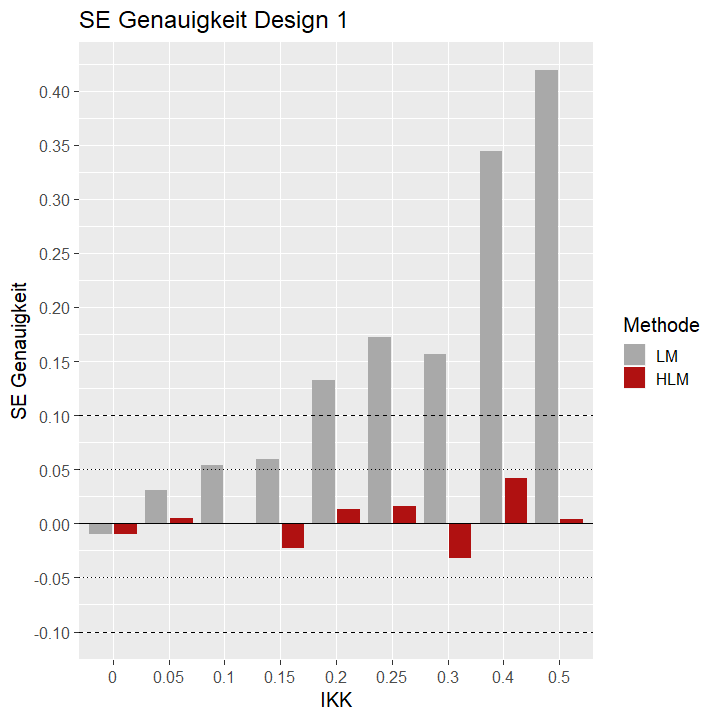
\includegraphics[width=8cm, height=8cm]{se_genauigkeit_design1}
\caption{Genauigkeit der Schätzung des Standardfehlers der Gesamtsteigung für jede Methode in allen IKK Bedingungen im ersten Simulationsdesign. SE: \textit{Standard Error}, LM: Lineares Modell, HLM: Hierarchisch lineares Modell, IKK: Intraklassen Korrelation}
\label{fig:se_genauigkeit_design1}
\end{figure}
In Abbildung \ref{fig:se_genauigkeit_design1} wird dieser Zusammenhang noch einmal graphisch dargestellt. Wie in Abbildung \ref{fig:se_genauigkeit_design1} zu erkennen und aus Tabelle \ref{tab:study1_results} zu entnehmen ist, bleiben die geschätzten Standardfehler des HLM immer hinnerhalb des akzeptablen Bereiches und erfüllen auch in allen Bedingungen das noch strengere Kriterium von $|\Delta\widehat{SE}_{\widehat{\gamma}}| > .05$. Die Schätzungen des Standardfehlers sind daher auch noch bei einer hohen IKK von .50 mit $\Delta\widehat{SE}_{\widehat{\gamma}_{10}} = .00$ im akzeptablen Bereich. Folglich kommt es bei der Analyse mit einem HLM zu keiner Unter- oder Überschätzung des Standardfehlers und führt dementsprechend zu keiner erhöhten Fehler Typ 1 oder Fehler Typ 2 Rate, die in einer tieferen Power resultiert.

Beim zweiten Simulationsdesign wurden die Standardfehler der Gesamtsteigung durch das LM mit einer Genauigkeit von $\Delta\widehat{SE}_{\widehat{\gamma}_{01}} = .0056$ bis $\Delta\widehat{SE}_{\widehat{\gamma}_{01}} = -.79$ geschätzt. Das HLM schätzte die Standardfehler mit einer Genauigkeit von $\Delta\widehat{SE}_{\widehat{\gamma}_{01}} = -.03$ bis $\Delta\widehat{SE}_{\widehat{\gamma}_{01}} = .04$. Beide Analysemethoden weisen wieder eine genaue Schätzung des Standardfehlers bei einer IKK von .00 auf. Betrachtet man die Entwicklung der Schätzung des Standardfehlers durch das LM, erkennt man, dass die Standardfehler wieder mit zunehmender IKK unterschätzt werden. Bei einer IKK von .05 wird mit $\Delta\widehat{SE}_{\widehat{\gamma}_{01}} = -.47$ der Grenzwert für eine akzeptable Abweichung bereits überschritten. Diese Unterschätzung steigt mit zunehmender IKK weiter an, bis hin zu einer SE Genauigkeit von $\Delta\widehat{SE}_{\widehat{\gamma}_{01}} = -.79$ bei einer IKK von 0.50. In diesem Fall resultiert diese Unterschätzung des Standardfehlers wieder in einer erhöhten Fehler Typ 1 Rate.
\begin{figure}[t!]
\centering
\captionsetup{width=8cm}
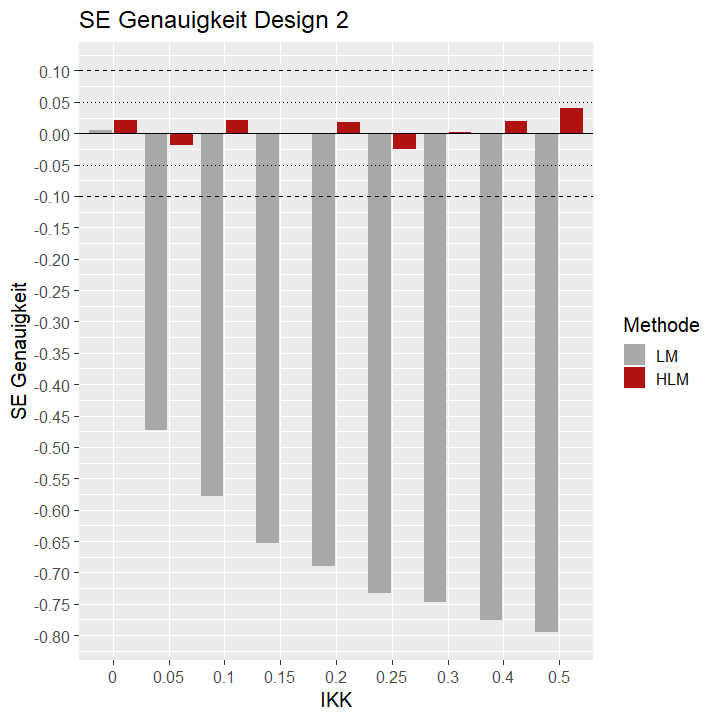
\includegraphics[width=8cm, height=8cm]{se_genauigkeit_design2}
\caption{Genauigkeit der Schätzung des Standardfehlers der Gesamtsteigung für jede Methode in allen IKK Bedingungen im zweiten Simulationsdesign. SE: \textit{Standard Error}, LM: Lineares Modell, HLM: Hierarchisch lineares Modell, IKK: Intraklassen Korrelation}
\label{fig:se_genauigkeit_design2}
\end{figure}
In Abbildung \ref{fig:se_genauigkeit_design2} sind wieder beide Verläufe über die verschiedenen IKK Bedingungen abgebildet. Dabei lässt sich zum einen direkt die Unterschätzung des Standardfehlers durch das LM erkennen, aber auch dass das HLM wieder eine sehr genaue Geschätzung des Standardfehlers aufweist. Diese Werte sind in der letzten Spalte der Tabelle \ref{tab:study1_results} abgebildet und zeigen, dass bei Verwendung von einem HLM die Standardfehler wieder in allen Bedingungen den Grenzwert von $|\Delta\widehat{SE}_{\widehat{\gamma}}| > .10$ nicht überschreiten und sogar kleiner als das noch strengere Kriterium $|\Delta\widehat{SE}_{\widehat{\gamma}}| > .05$ sind. Es entsteht folglich wieder weder eine Unter- noch Überschätzung des Standardfehlers bei der Verwendung eines HLM in diesem Simulationsdesign und dies resultiert demnach in keiner erhöhten Fehler Typ 1 oder Fehler Typ 2 Rate.

\subsubsection{Diskussion Studie 1}
Mit der ersten Studie dieser Arbeit wurde überprüft, wie sich die Schätzgenauigkeit von Regressionskoeffizienten und Standardfehlern zwischen LM und HLM bei der Analyse von hierarchischen Daten unterscheidet, wie sich diese Schätzungen bei variierender IKK verhalten und ob die Ebene der Intervention einen Einfluss auf die Schätzgenauigkeit hat. 

Dabei konnte gezeigt werden, dass beide Methoden die Regressionskoeffizienten des Gesamtmittelwertes und der Gesamtsteigung über alle Bedingungen genau schätzten. Unterschiede in der Schätzgenauigkeit gab es erst bei der Schätzung der Standardfehler. So wurde der Standardfehler des Gesamtmittelwertes bei steigender IKK in beiden Simulationsdesigns bei Verwendung von LM zunehmend unterschätzt. Nur bei einer IKK von .00 schätzte das LM den Standardfehler genau. Das bedeutet, dass ein LM den Standardfehler nur dann genau schätzt, wenn die zwischen den Gruppen keine zufällige Abweichung besteht und die Gruppenzugehörigkeit folglich keinen Einfluss auf die abhängige Variable hat. Das HLM schätzte hingegen in allen Bedingungen und in beiden Simulationsdesigns die Standardfehler des Gesamtmittelwertes genau. Bei der Schätzung des Standardfehlers der Gesamtsteigung gab es bei der Verwendung von LM einen Unterschied bezüglich des Simulationsdesigns. Im ersten Simulationsdesign mit einem Level-1 Prädiktor wurde sobald die Gruppenzugehörigkeit einen Einfluss hatte, der Standardfehler mit steigender IKK zunehmend überschätzt. Beim zweiten Simulationsdesign mit einem Level-2 Prädiktor wurde der Standardfehler bei steigender IKK zunehmend unterschätzt. Bei der Analyse mittels HLM wurden wieder in allen Bedingungen und in beiden Simulationsdesigns die Standardfehler der Gesamtsteigung genau geschätzt.

Diese Ergebnisse bedeuten, dass es je nach Fokus der Forschungsfrage einen entscheidenden Einfluss hat, ob man ein LM oder ein HLM verwendet. Interessiert man sich nur für die Ausprägung der Regressionskoeffizienten spielt die Wahl der Analysemethode also keine grosse Rolle. Zu dieser Erkenntnis kamen auch schon Autoren aus früheren Studien \citep{mcneish2014analyzing, mundfrom2002monte, osborne2000advantages} und diese wurde mit der vorliegenden Simulationsstudie noch einmal gestützt. 

Eine weitere Schlussfolgerung, die aus diesen Ergebnissen gezogen werden kann, ist dass es sich empfiehlt hierarchische Daten mittels HLM zu analysieren um Ungenauigkeiten in der Schätzung des Standardfehlers und schlussendlich höhere Fehler Typ 1 oder Fehler Typ 2 Raten zu verhindern. Werden trotz dem Vorhandensein hierarchischer Strukturen mit LM gearbeitet, kann es je nach Studiendesign zu massiven Unter- oder Überschätzung der Standardfehler kommen und folglich zu verzerrten Studienergebnissen führen. Bei einer Unterschätzung des Standardfehlers laufen gemäss dieser Ergebnisse Forschende Gefahr, aufgrund der erhöhten Fehler Typ 1 Rate Effekte zu finden, die in Wahrheit gar nicht vorhanden sind. Diese Unterschätzung tritt vor allem dann auf, wenn Interventionen auf Level-2 durchgeführt werden und wurde ebenfalls bereits von Moerbeek et al. \citeyearpar{MOERBEEK2003341} mathematisch aufgezeigt. Zu einer Überschätzung des Standardfehlers und folglich zu einer erhöhten Fehler Typ 2 Rate kommt es, wenn bei einer Intervention auf Level-1 die hierarchische Struktur missachtet und mit einem LM analysiert wird. Dabei spielt es gemäss Moerbeek et al. \citeyearpar{MOERBEEK2003341} eine Rolle, ob von einer Interaktion zwischen Intervention und Gruppenzugehörigkeit ausgegangen wird oder nicht. Wird von keiner Interaktion ausgegangen, wie in unserer Simulationsstudie, werden Standardfehler von LM zunehmend überschätzt. Wird hingegen bei der Anaylse eine Interaktion zwischen Intervention und Gruppenzugehörigkeit angenommen, kann es in Abhängigkeit der Varianzkomponenten und der Gruppengrössen zu einer Unter- oder Überschätzung des Standardfehlers führen \citep{MOERBEEK2003341}. 

Bis jetzt wurden allerdings nur die Schätzgenauigkeit der Regressionskoeffizienten und der Standardfehler besprochen und nicht die Fehlerraten oder die effektive Power dieser beiden Analysemethoden. Auch wenn aufgrund der Ergebnisse aus der ersten Simulationsstudie hervorgeht, dass eine Verwendung von HLM bei der Analyse von hierarchischen Daten zu genaueren Schätzungen und weniger Verzerrung der Prüfgrösse führt als LM, wäre es interessant zu beobachten wie sich die Fehlerraten und die Power dieser beiden Methoden über die verschiedenen IKK Bedingungen verändert. 

\subsection{Studie 2: Zuverlässigkeit von LM und HLM}
In der zweiten Studie wurde untersucht, wie zuverlässig LMs und HLMs einen Effekt einer Intervention finden. Die Fehler Typ 1 Rate und die Power sind zwei mögliche Indikatoren für diese Zuverlässigkeit einer Methode. Wie bereits erwähnt, entsteht ein Fehler Typ 1 dann, wenn ein Test fälschlicherweise zu einem signifikanten Ergebnis gelangt. Das würde beispielsweise bedeuten, dass ein Test eine Intervention als effektiv identifiziert, obwohl sie das in Wirklichkeit gar nicht ist. Die Power bezeichnet die Fähigkeit einen Effekt zu finden, wenn er auch wirklich vorhanden ist. Damit die Fehler Typ 1 Rate als auch die Power untersucht werden kann, wurden in dieser Simulationsstudie die Datensätze einmal mit einer effektiven Intervention und einmal mit einer ineffektiven Intervention simuliert. Unter einer ineffektiven Intervention wird hier eine Intervention verstanden, die keinen Effekt auf die abhängige Variable hat. Das bedeutet, dass bei der Simulation der ineffektiven Intervention die Gesamtsteigung des Level-1 Prädiktors $\gamma_{10}$ und die des Level-2 Prädiktors $\gamma_{10}$ auf 0 gesetzt wurden. Betrachtet man die Gleichungen aus Abschnitt \ref{section:sim_design}, kann man erkennen, dass mit diesen gewählten Werten für $\gamma_{10}$ bzw. $\gamma_{10}$ die Level-1 Variable $x_{ij}$ bzw. die Level-2 Variable $z_{j}$ keinen Einfluss mehr auf die Ausprägung der abhängigen Variable $y_{ij}$ hat.

Die Fehlerraten und die Power stehen in einem direkten Zusammenhang mit der Stichprobengrösse, so dass eine steigende Stichprobengrösse zu einer tieferen Fehlerrate und einer höheren Power führt \citep{snijders2005samplesizepower}. Folglich würde eine so grosse Stichprobe aus Studie 1 wahrscheinlich zu keinen Unterschieden in den Fehlerraten oder der Power zwischen den beiden Methoden führen. Allerdings ist es in der Praxis oft nicht möglich, eine solche grosse Stichprobe von insgesamt 15000 Beobachtungen zu erheben. Daher wurde in dieser zweiten Studie eine etwas reduzierte und praxisnähere Stichprobengrösse für die beiden Studiendesigns simuliert. Die Anzahl simulierter Klassen wurde folglich auf 70 und die Klassengrösse auf 12 reduziert. Diese Werte entsprechen nun  den festgelegten Werte aus der Simulation von Moerbeek et al. \citeyearpar{MOERBEEK2003341}, die aus dem Datensatz des \textit{TVSFP} entnommen wurden \citep{FLAY1995smoking}. Diese Reduktion führte zu einer Stichprobengrösse von insgesamt 840 Beobachtungen. 

Wie bereits in der Herleitung der Forschungsfrage beschrieben, wurde der Effekt der Intervention mit einem \textit{t} Test überprüft, dessen Prüfgrösse sich aus dem Verhältnis des Geschätzten Regressionskoeffizienten und dem dazugehörigen Standardfehler berechnet. Die Anzahl Freiheitsgrade wurde bei normalen linearen Modellen mittels der bekannten Formel $N - p - 1$ berechnet. Bei den hierarchischen linearen Modellen wurde die Satterthwaite Methode verwendet, um die Anzahl Freiheitsgrade zu bestimmen \citeyearpar{satter1941synthesis}. Die Satterthwaite Methode ist eine der in der Forschung diskutierten Methoden, die häufig zur Berechnung der Freiheitsgrade von hierarchischen linearen Modellen verwendet wird \citep{raudenbush2002hierarchical,SnijdersTomA.B2012Ma:a}. 

Um nun die Fehlerraten und die Power zu berechnen, wurde für alle Datensätze in jeder Bedingung und für jede Analysemethode die Anzahl an Tests, die auf einem Signifikanzniveau von 5\% signifikant wurden, durch die Anzahl Replikationen pro Bedingung geteilt. Dies ergibt die prozentuale Häufigkeit, bei der die Analysemethode in der gegebenen IKK Bedingung einen signifikanten Effekt gefunden hat. In einem Datensatz mit einer effektiven Intervention entspricht diese prozentuale Häufigkeit der Power. In einem Datensatz mit einer ineffektiven Intervention gibt diese Häufigkeit der Fehler Typ 1 Rate an.

\subsubsection{Ergebnisse Studie 2}
Die Ergebnisse der zweiten Simulationsstudie werden in Tabelle \ref{tab:power_study2} abgebildet. Es ist zu beachten, dass die Fehler Typ 1 Rate und die Power nur für die Gesamtsteigung des Level-1 Prädiktors $\widehat{\gamma}_{10}$ bzw. die des Level-2 Prädiktors $\widehat{\gamma}_{10}$ berechnet wurde, weil diese Regressionskoeffizienten auch den Effekt der Intervention abbilden. Als erstes werden die Datensätze besprochen, die mit $\widehat{\gamma}_{10} = 0.12$ bzw. $\widehat{\gamma}_{10} = 0.12$ simuliert wurden. Dies entspricht hier einer effektiven Intervention und wird folglich dazu verwendet, um die Power der beiden Methoden zu untersuchen.

Im ersten Simulationsdesign in dem die Intervention auf Level-1 durchgeführt wurde, reicht die Power des LM von $.44$ bis $.76$. Dabei ist zu beachten, dass bei einer IKK von .00 die höchste Power von $.76$ erreicht wird und mit zunehmender IKK abnimmt.
\begin{table}[t!]
\centering
\setlength{\tabcolsep}{10pt}
\begin{threeparttable}
\caption{Power und Fehler Typ 1 Rate in beiden Simulationsdesigns für jede Analysemethode in allen IKK Bedingungen.}
\begin{tabular}{lcccccccc}
\toprule
	& \multicolumn{4}{c}{Power} & \multicolumn{4}{c}{Fehler Typ 1 Rate}\\
\cmidrule(lr){2-5} \cmidrule(lr){6-9}
	& \multicolumn{2}{c}{Design 1} 
	& \multicolumn{2}{c}{Design 2} 
	& \multicolumn{2}{c}{Design 1} 
	& \multicolumn{2}{c}{Design 2}\\
\cmidrule(lr){2-3} \cmidrule(lr){4-5} \cmidrule(lr){6-7} \cmidrule(lr){8-9}
IKK & LM  & HLM & LM  & HLM & LM   & HLM & LM  & HLM\\ 
\midrule
.00 & .76 & .76 & .74 & .72 & .05  & .05 & .05 & .04\\
.05 & .72 & .75 & .71 & .53 & .05  & .06 & .12 & .06\\
.10 & .73 & .76 & .64 & .38 & .04  & .05 & .17 & .05\\
.15 & .72 & .78 & .64 & .34 & .04  & .05 & .23 & .05\\
.20 & .67 & .75 & .56 & .24 & .02  & .04 & .27 & .04\\
.25 & .69 & .78 & .56 & .21 & .02  & .05 & .29 & .04\\
.30 & .62 & .78 & .57 & .19 & .02  & .05 & .36 & .06\\
.40 & .55 & .77 & .56 & .13 & .01  & .05 & .43 & .06\\
.50 & .44 & .76 & .55 & .10 & .01  & .06 & .46 & .04\\
\bottomrule
\end{tabular}
\label{tab:power_study2}
\begin{tablenotes}[flushleft]
\footnotesize
\item
Hinweis: Bei Power wurden Datensätze mit einer Gesamtsteigung von $\widehat{\gamma}_{10} = 0.12$ bzw. $\widehat{\gamma}_{10} = 0.12$ simuliert. Bei der Fehler Typ 1 Rate mit $\widehat{\gamma}_{10} = 0$ bzw. $\widehat{\gamma}_{10} = 0$. IKK: Intraklassenkorrelation, LM: Lineares Modell, HLM: Hierarchisch lineares Modell
\end{tablenotes}
\end{threeparttable}
\end{table} 
In Abbildung \ref{fig:results_power} sind auf der linken Seite die einzelnen Power-Werte jeder IKK Bedingung und für jede Analysemethode abgebildet. Dabei lässt sich erkennen, dass die Power von einem LM bis zu einer IKK von .10 noch einigermassen mit der Power eines HLMs mithalten kann. Sobald aber die IKK grösser als .10 ist lässt sich eine kontinuierliche Abnahme der Power beobachten. Betrachtet man die Schätzgenauigkeit des Standardfehlers des LMs an dieser Stelle, erkennt man, dass ab einer IKK von .15 mit $\Delta\widehat{SE}_{\widehat{\gamma}_{10}} = 0.1167$ den Grenzwert von $|\Delta\widehat{SE}_{\widehat{\gamma}}| > .10$ \citep{hooglandboosma1998robustness} überschritten wird und folglich die Schätzung des Standardfehlers als nicht mehr akzeptabel gilt. Dies führt zu einer zu hohen Fehler Typ 2 Rate, die schlussendlich  in dieser tieferen Power resultiert. Die Power unter Verwendung des HLMs reicht von $.75$ bis $.78$ und bleibt gemäss Abbildung \ref{fig:results_power} über alle Bedingungen relativ konstant. Die Schätzgenauigkeit der Standardfehler mittels HLM überschreitet in keiner IKK Bedingung den Grenzwert von $|\Delta\widehat{SE}_{\widehat{\gamma}}| > .10$. Bei einer Analyse mit einem HLM kommt es in diesem Fall also weder zu einer Über- noch einer Unterschätzung des Standardfehlers.

Im zweiten Simulationsdesign bei dem die Intervention auf Level-2 durchgeführt wurde, reicht die Power des LMs von $.55$ bis $.74$ und nimmt wieder mit steigender IKK ab. Die Power des HLMs reicht im zweiten Simulationsdesign von $.10$ bis $.72$ und verzeichnete ebenfalls eine Abnahme der Power mit zunehmender IKK. Auf der rechten Seite der Abbildung \ref{fig:results_power} ist dieser Verlauf noch einmal Visualisiert. Dabei kann man erkennen, dass die Abnahme der Power bei einer zunehmenden IKK bei einer Analyse mit einem HLM stärker als bei einer Analyse mit einem LM ist. Bei einer IKK von $.50$ erreichte ein HLM nur noch eine Power von $.10$, wobei ein LM eine Power von $.55$ erreichte. Die Schätzgenauigkeiten des Standardfehlers werden ähnlich wie in Studie 1 von dem LM ab einer IKK von .05 stark unterschätzt und überschreiten in allen weiteren IKK Bedingungen den Grenzwert von $|\Delta\widehat{SE}_{\widehat{\gamma}}| > .10$. Diese Unterschätzung der Standardfehler durch das LM führt zu einer Inflation der Prüfgrösse und schlussendlich zu dieser vermeintlich besseren Power. Die Schätzung der Standardfehler bleibt bei der Verwendung eines HLMs im akzeptablen Bereich und überschreiten den Grenzwert in keiner IKK Bedingung. Folglich bildet ein HLM in dieser Situation die Power adäquater als ein LM ab.

\begin{figure}[t!]
\centering
\captionsetup{width=\textwidth}
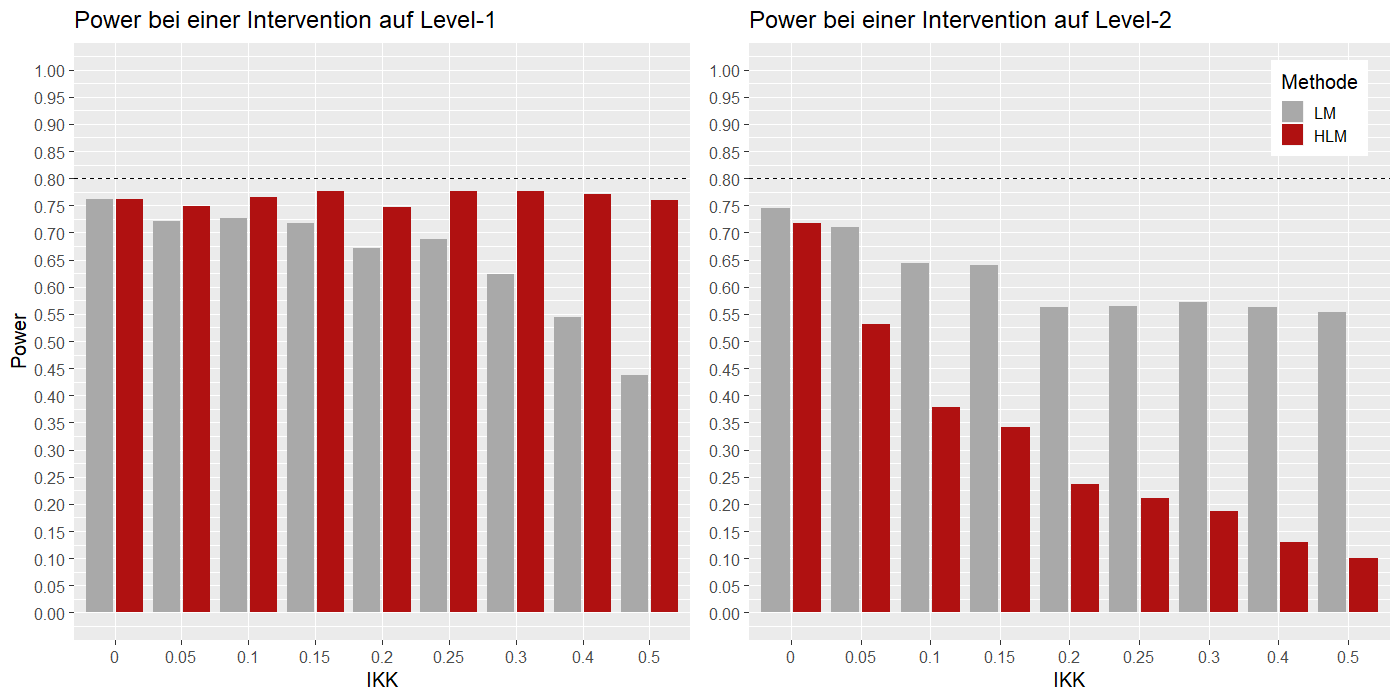
\includegraphics[width = \textwidth]{results_power}
\caption{Statistische Power von LM und HLM in den verschiedenen IKK Bedingungen in beiden Studiendesigns. LM: Lineares Modell, HLM: Hierarchisches lineares Modell}
\label{fig:results_power}
\end{figure}

Die im Anschluss besprochenen Ergebnisse, beziehen sich auf die simulierten Datensätze mit einer ineffektiven Intervention, die mit einer Gesamtsteigung von $\widehat{\gamma}_{10} = 0$ bzw. $\widehat{\gamma}_{10} = 0$ simuliert wurden. In den letzten vier Spalten der Tabelle \ref{tab:power_study2} sind die Fehler Typ 1 Raten beider Simulationsdesigns aufgeführt. Im ersten Simulationsdesign mit einer Intervention auf Level-1, zeigt sich, dass die Fehler Typ 1 Rate bei einem LM mit zunehmender IKK fortlaufend abnimmt. Diese Reduktion der Fehler Typ 1 Rate von $.05$ auf $0.01$ ist auf die Überschätzung des Standardfehlers in diesem Studiendesign zurückzuführen. Die Fehler Typ 1 Rate des HLMs im ersten Studiendesign reicht von $.04$ bis $.06$. Diese Entspricht ungefähr den Erwartungen, die man bei einem Signifikanzniveau von 5\% hat.

Betrachtet man nun die Fehler Typ 1 Raten des zweiten Studiendesigns, kann man erkennen, dass die Fehler Typ 1 Rate des LMs mit zunehmender IKK von $.05$ bis $.46$ ansteigt. Dieser Anstieg der Fehler Typ 1 Rate ist auf die Inflation der Prüfgrösse zurückzuführen, die aufgrund der Unterschätzung des Standardfehlers entsteht. Bereits ab einer IKK von $.05$ wird mit $.12$ das Signifikanzniveau von 5\% überschritten. Im Vergleich dazu liegen die Fehler Typ 1 Raten des HLMs wieder in einem Bereich von $.04$ bis $.06$. In Abbildung \ref{fig:results_error_lvl2} ist der Verlauf der Fehler Typ 1 Raten von LMs und HLMs noch einmal visualisiert. 

\begin{figure}[t!]
\centering
\captionsetup{width=8cm}
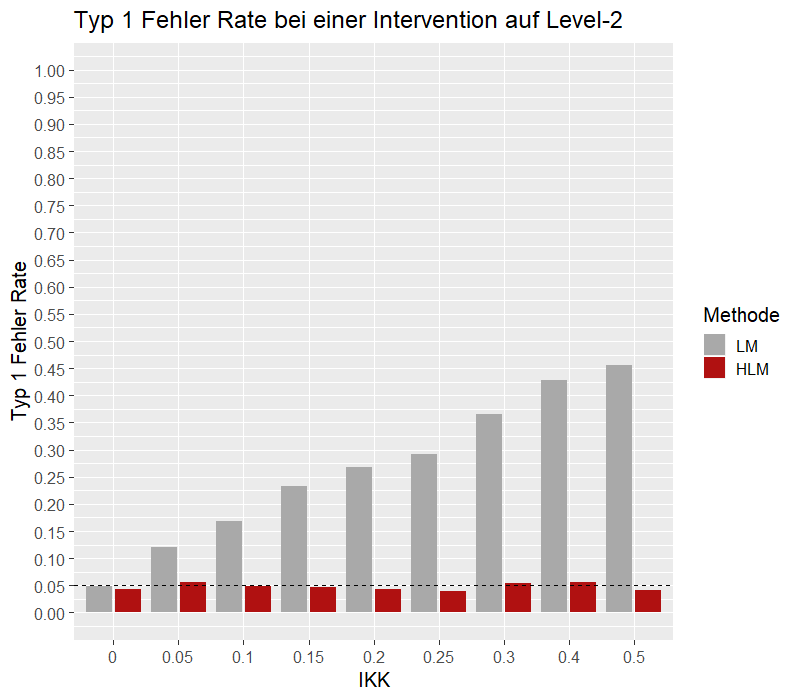
\includegraphics[width=8cm, height=8cm]{results_error_lvl2}
\caption{Fehler Typ 1 Rate von LMs und HLMs bei einer ineffektiven Intervention auf Level-2. LM: Lineares Modell, HLM: Hierarchisches lineares Modell}
\label{fig:results_error_lvl2}
\end{figure}

\subsubsection{Diskussion Studie 2}
Die zweite Simulationsstudie untersuchte, wie genau sich die Fehlerraten und die Power bezüglich eines Effekts einer Intervention zwischen den beiden Analysemethoden unterscheidet und vor allem wie sich diese beiden Faktoren über die verschiedenen IKK Bedingungen verändern. Wie in der ersten Studie wurde auch in der zweiten Studie zwischen zwei Simulationsdesigns unterschieden bei denen die Intervention zum einen auf Level-1 und zum anderen auf Level-2 durchgeführt wurde.

Im ersten Studiendesign bestätigte sich die Vermutung aus der vorherigen Studie, dass bei einer Intervention auf Level-1 ohne Interaktion zwischen Gruppenzugehörigkeit und Intervention die Power mit zunehmender IKK abnimmt, wenn bei der Analyse ein LM verwendet wird. Wird an Stelle von einem LM ein HLM verwendet bleibt die Power über alle IKK Bedingungen konstant. Im zweiten Simulationsdesign zeigte sich allerdings eine Abnahme der Power bei beiden Analysemethoden bei zunehmender IKK. Diese Abnahme war bei der Verwendung von LM geringer als bei der Verwendung von HLM. Vergleicht man die Fehler Typ 1 Raten dieser beiden Modelle, bestätigten sich ebenfalls die Erwartungen. Im ersten Studiendesign nahmen die Fehler Typ 1 Rate des LMs aufgrund der zunehmenden Überschätzung des Standardfehlers bei ansteigender IKK fortlaufend ab. Genau das gegenteilige Bild zeigte sich beim zweiten Studiendesign. Hier stieg die Fehler Typ 1 Rate des LMs bei zunehmender IKK stark an. Die Fehler Typ 1 Rate des HLMs blieb in beiden Studiendesign in einem akzeptablen Bereich. 

Interessiert man sich nun für den Effekt einer Intervention, lässt sich aus diesen Ergebnissen zwei Schlussfolgerungen ziehen. Zum einen ist es ratsam, wenn immer möglich die Intervention auf Level-1 durchzuführen, da die Power im zweiten Simulationsdesign bei beiden Analysemethoden mit steigender IKK stark abnahm. Diese Erkenntnis stimmt mit den Aussagen aus der Literatur überein, dass eine Intervention auf Level-2 es erschwert, den Effekt der Intervention von dem Effekt der Gruppenzugehörigkeit zu trennen, da in diesem Studiendesign keine Beobachtungen aus Kontroll- und Interventionsgruppe in der selben Level-2 Einheit vorhanden sind \citep{cleary2012studydesign, moerbeek2000design}. 

Zum anderen sollte grundsätzlich ein HLM zur Analyse von hierarchischen Daten verwendet werden, da sich die Power bei einer Intervention auf Level-1 auch bei hoher IKK nicht verschlechtert. Ist es den Forschenden jedoch nicht möglich eine Intervention auf Level-1 durchzuführen, sollte man sich nicht von den Ergebnissen auf der rechten Seite der Abbildung \ref{fig:results_power} täuschen lassen. Auch wenn es so scheint, dass ein LM eine weniger starke Reduktion der Power erfährt als ein HLM, sollte in dieser Situation trotzdem ein HLM zur Analyse verwendet werden. Da in der ersten Studie gezeigt wurde, dass in dieser Situation der Standardfehler von einem LM stark unterschätzt wird, kann diese schwache Abnahme der Power auf die Inflation der Prüfgrösse und die Zunahme der signifikanten Tests zurückgeführt werden. Diese Unterschätzung des Standardfehlers und die Inflation der Prüfgrösse ist vor allem bei der Fehler Typ 1 Rate in Abbildung \ref{fig:results_error_lvl2} gut zu beobachten. Obwohl die Intervention in dieser Studienanordnung keinen Effekt auf die abhängige Variable hatte, gelang es dem LM bei zunehmender IKK schlechter den Standardfehler genau zu schätzen und fand schlussendlich bei einer IKK von .50 in fast der Hälfte aller Fälle einen fälschlicherweise signifikanten Effekt der Intervention.

Da es bei der Analyse mittels HLM zu keiner Verzerrung der Schätzung des Standardfehlers kommt, kann der Power von HLM mehr Vertrauen geschenkt werden. Mit dieser Information könnten nun Forschende die Analysemethode als Ursache für diese tiefe Power ausschliessen und nach anderen Gründe suchen, die zu dieser tiefen Power führen (z.B. Studiendesign oder Stichprobengrösse).

\subsection{Abschliessende Diskussion und Shiny App}
Mit diesen beiden Studien wurde das Ziel verfolgt, die Unterschiede zwischen der Schätz-genauigkeit von Regressionskoeffizienten und deren Standardfehlern sowie die daraus resultierende Fehler Typ 1 Rate und Power von LMs und HLMs zu untersuchen. Auch wenn die Regressionskoeffizienten von beiden Methoden genau geschätzt wurden, konnten die Studien zeigen, dass ein HLM auch bei hoher Abhängigkeit der Gruppenzugehörigkeit genaue Schätzungen der Standardfehler liefert, wohingegen ein LM bei steigender IKK eine immer stärkere Verzerrung der Schätzung aufweist. Dementsprechend führten Analysen mit einem HLM auch zu keiner Verzerrung der Power bei der Testung von Interventionseffekten.

Die aus dieser Simulationsstudie resultierende Erkenntnis, dass ein HLM einen klaren Vorteil gegenüber einem LM bei der Analyse von hierarchischen Daten vorweisen, ist keine Neuheit und wurde in einigen Studien bereits gefunden \citep{mcneish2014analyzing, MOERBEEK2003341, mundfrom2002monte, osborne2000advantages}. Dennoch konnte diese Studie, die in Moerbeek et al. \citeyearpar{MOERBEEK2003341} verwendeten Studiendesigns in eine Simulationsstudie integrieren, um den Einfluss dieser beiden Interventionsformen auf die Schätzgenauigkeit von LMs und HLMs zu untersuchen. Damit können klare Empfehlungen für die Forschung mit hierarchischen Daten abgeleitet werden. Beispielsweise sollte wenn immer möglich eine Intervention auf Level-1 durchgeführt werden, um Effekte der Gruppenzugehörigkeit von Effekten der Intervention trennen zu können. 

In manchen Fällen ist es allerdings nicht möglich die Intervention auf Level-1 durchzuführen und benötigen daher eine Intervention auf Level-2, um eine Kontamination der Interventionsgruppe zu vermeiden. Ein Beispiel dafür wären Interventionen mit Familien, bei denen es schwierig ist gewisse Interventionen nur bei einzelne Familienmitgliedern durchzuführen, ohne dass andere Familienmitglieder davon beeinflusst werden. Wie man in der zweiten Studie beobachten konnte, verringerte sich die Power des HLMs bei einer Intervention auf Level-2 bei einer Zunahme der IKK enorm. Weiterführende Simulationsstudien könnten nun untersuchen, welche Möglichkeiten es gibt diese Power zu verbessern. Da in der aktuellen Simulationsstudie nur die IKK variiert wurde, die Power aber mit steigender Stichprobengrösse zunimmt, könnten weitere Studien untersuchen, wie gross eine Stichprobe sein müsste, damit ein HLM auch bei einer Intervention auf Level-2 eine akzeptable Power liefert. Dabei könnte ebenfalls untersucht werden, ob es ein optimales Verhältnis zwischen Gruppengrösse und Gruppenanzahl gibt, um die Power eines HLMs zu maximiere.

Die aktuelle Studie unterlag mehreren Limitationen. Zum einen wurde nur ein sehr einfaches Modell zur Simulation der Daten verwendet. Dabei gab es keine \textit{Cross-Level} Interaktion zwischen einem Level-1 und einem Level-2 Prädiktor. Da in realen Datensätzen solche \textit{Cross-Level} Interaktion wahrscheinlich vorhanden sind, können Ergebnisse aus dieser Simulationsstudie nicht auf solche Situationen angewandt werden. Daher wäre es interessant, wenn weitere Simulationsstudien \textit{Cross-Level} Interaktionen in Bezug auf diese Aufteilung in zwei Interventionsdesigns untersuchen könnten. Eine weitere Limitation dieser Simulationsstudie ist, dass nur die IKK variiert wurde. So erhält man zwar einen Einblick, wie sich die Messmethode über verschiedene Einflussstärken der Gruppenzugehörigkeit verhält, es gibt aber keine Einsicht darüber, wie gross eine Stichprobe gewählt werden sollte, um eine genaue Schätzung und eine akzeptable Power zu erhalten. Da die Wahl der Stichprobengrösse in der Forschung oft eine Kostenfrage ist, könnte durch eine weitere Simulationsstudie, die diese Punkte berücksichtigt, klare Empfehlungen für die Praxis erarbeitet werden. Als abschliessende Limitation kann die Wahl des Grenzwertes für die Schätzgenauigkeit des Standardfehlers genannt werden. Dieser Grenzwert von $|\Delta\widehat{SE}_{\widehat{\gamma}}| > .10$ wurde von Hoogland und Boosma \citeyearpar{hooglandboosma1998robustness} festgelegt. Wie man aber auf der linken Seite der Abbildung \ref{fig:results_power} erkennen kann, sinkt die Power eines LMs bereits bei einer IKK von .05. Bei dieser IKK wird bereits die Schätzgenauigkeit von $|\Delta\widehat{SE}_{\widehat{\gamma}}| > .05$ überschritten. Weitere Simulationsstudien könnten untersuchen, ob dieser Grenzwert von $|\Delta\widehat{SE}_{\widehat{\gamma}}| > .10$ gerechtfertigt ist oder ob ein strengerer Grenzwert benötigt wird, um genaue von ungenauen Analysemethoden zu trennen.

Die Ergebnisse dieser Simulationsstudie und eine kleine Einführung zu HLM können in einer interaktiven Form in der im Laufe dieser Arbeit programmierten Shiny App abgerufen werden. Dabei wurde die Shiny App ebenfalls in zwei Teile unterteilt, wobei der erste Teil sich der Theorie widmet und Nutzer selber einen hierarchischen Datensatz generieren, den sie dann mit LM oder HLM analysieren können. Für jede Analysemethode werden Regressionsgeraden, Residuenplots, Q-Q Plots abgebildet, damit die Nutzer einen direkten Vergleich dieser Methoden erhalten. Im zweiten Teil der Shiny App wird kurz die Forschungsfrage und das Studiendesign vorgestellt und anschliessend können die Nutzer für jede Teilstudie die Ergebnisse jeder Bedingung anzeigen lassen und erhalten dazu in einer Infobox die dazugehörige Erklärungen und Implikationen. Die im Anhang aufgeführten Screenshots geben eine weitere Übersicht über den hier kurz vorgestellten Aufbau und Inhalt der Shiny App.

Die aktuelle Studie konnte zeigen, dass es sich bei hierarchischen Daten und einem geeigneten Interventionsdesign lohnt ein HLM anstelle eines LMs zu verwenden, da dieses Modell die nötigen Parameter genau schätzen und zu einer konstanten Power führen. Ebenfalls konnte gezeigt werden, dass bei der Verwendung eines HLMs die Fehler Typ 1 Rate konstant gehalten werden kann, auch wenn der Einfluss der Gruppenzugehörigkeit ansteigt. Dies gibt Forschenden mehr Sicherheit bei der Testung von Effekten und führt zu glaubhafteren Ergebnissen. Zukünftige Simulationsstudien könnten sich mit weiteren Aspekten beschäftigen, die einen Einfluss auf die Schätzgenauigkeit haben.





\newpage
\singlespacing

\bibliography{literatur_masterarbeit}
\bibliographystyle{apacite}

\section{Anhang}
\appendix
\section{Shiny App Screenshots}
\section{R Code}





\end{document}
